\documentclass[12pt,a4paper]{article}
\input{~/template/report/preamble.tex}
\author{ZHANGYIHENG 10.7 27}
\title{Circular Motion}
\date{}
\begin{document}
\setmainfont{Times New Roman}
\setsansfont{Times New Roman}
\begin{spacing}{1.25}
\maketitle
\tableofcontents
\setlength{\parindent}{4ex}
\newpage
\section{Introduction}
\subsection{Circular Motion}
Circular motion refers to the motion of an object that moves along a circular path. In circular motion, an object moves with a constant speed around a fixed point or axis without changing its distance from the center. 
\subsection{Aim of the Experiment}
To find the relationship between $ t $(Time) and $ v $(Linear Velocity) when there exists a angular acceleration($ \alpha $)
\subsection{Apparatuses}
\begin{enumerate}
    \setlength{\itemsep}{-1ex}
    \setlength{\parsep}{-1ex}
    \setlength{\topsep}{-1em}
    \item laptop
    \item https://phet.colorado.edu/en/simulations/legacy/rotation
\end{enumerate}
\section{Data Collection}
\subsection{Procedure}
Simulate with the software.\par
All the data are recorded in the raw data table.
\subsection{Screenshots}
\begin{figure}[H]
    \centering  %图片全局居中
    \subfigure[0$ s $]{
    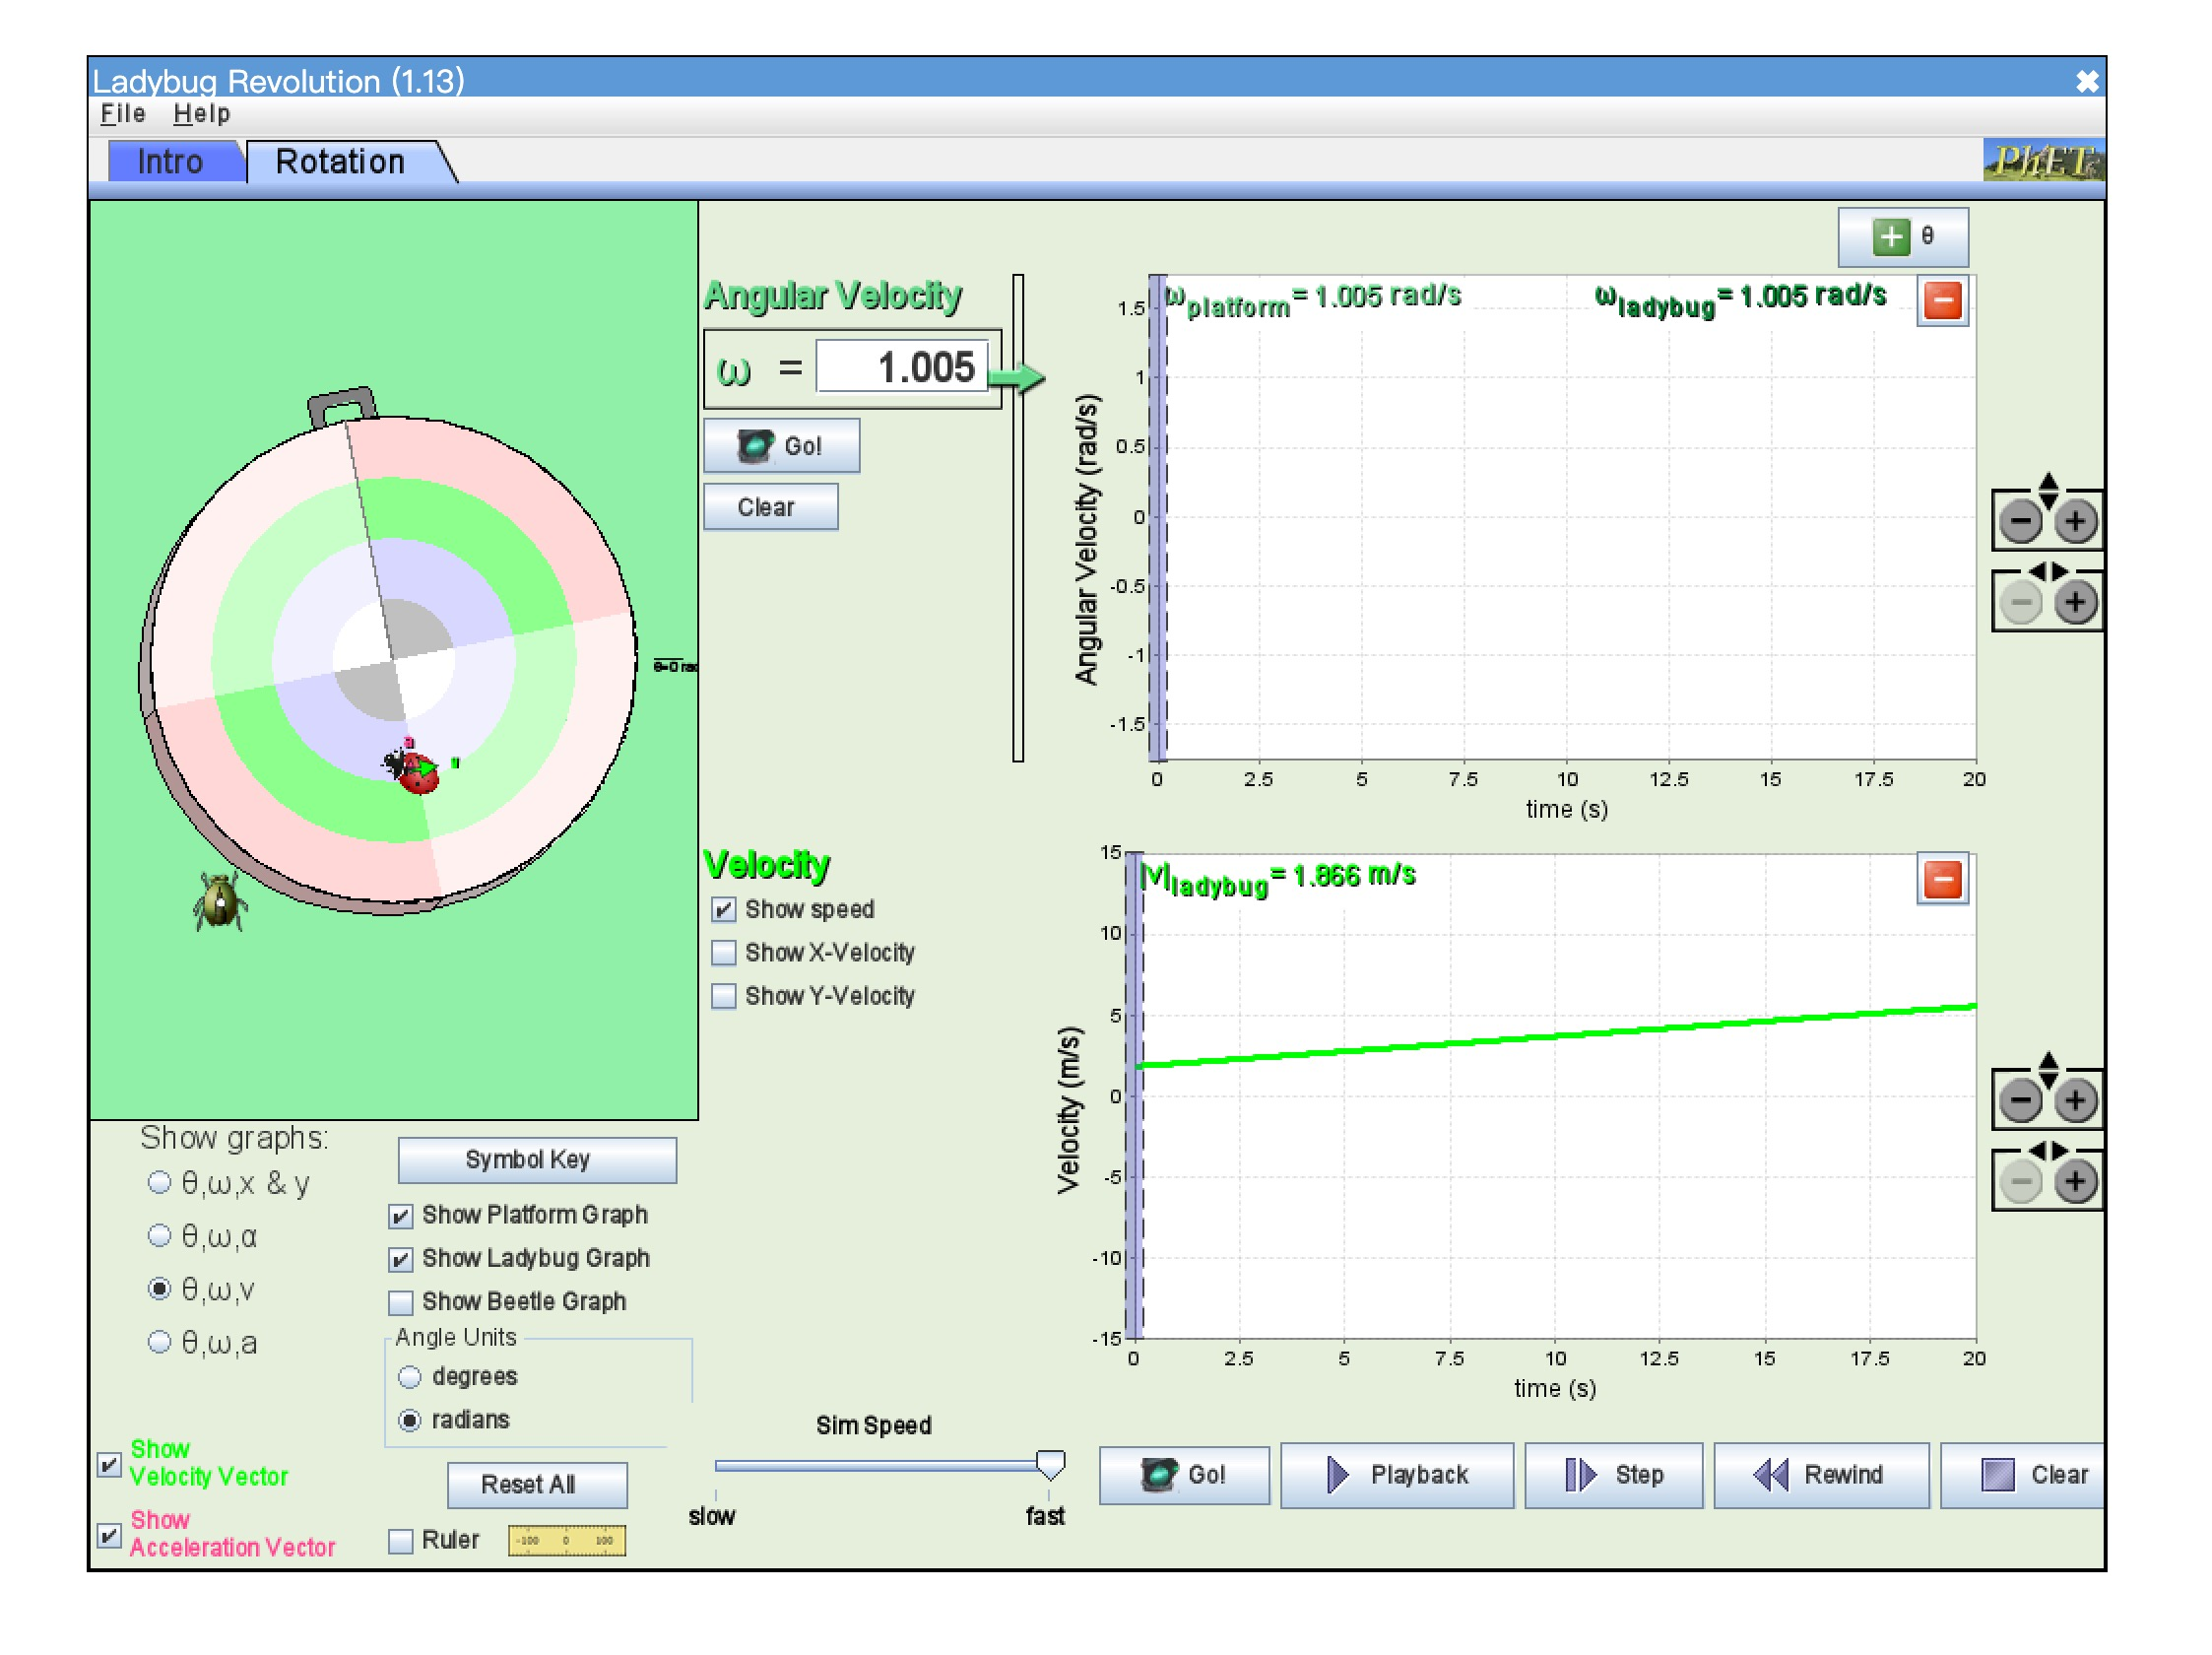
\includegraphics[width=0.3\textwidth]{1.jpeg}}
    \subfigure[$ 2.50s $]{
    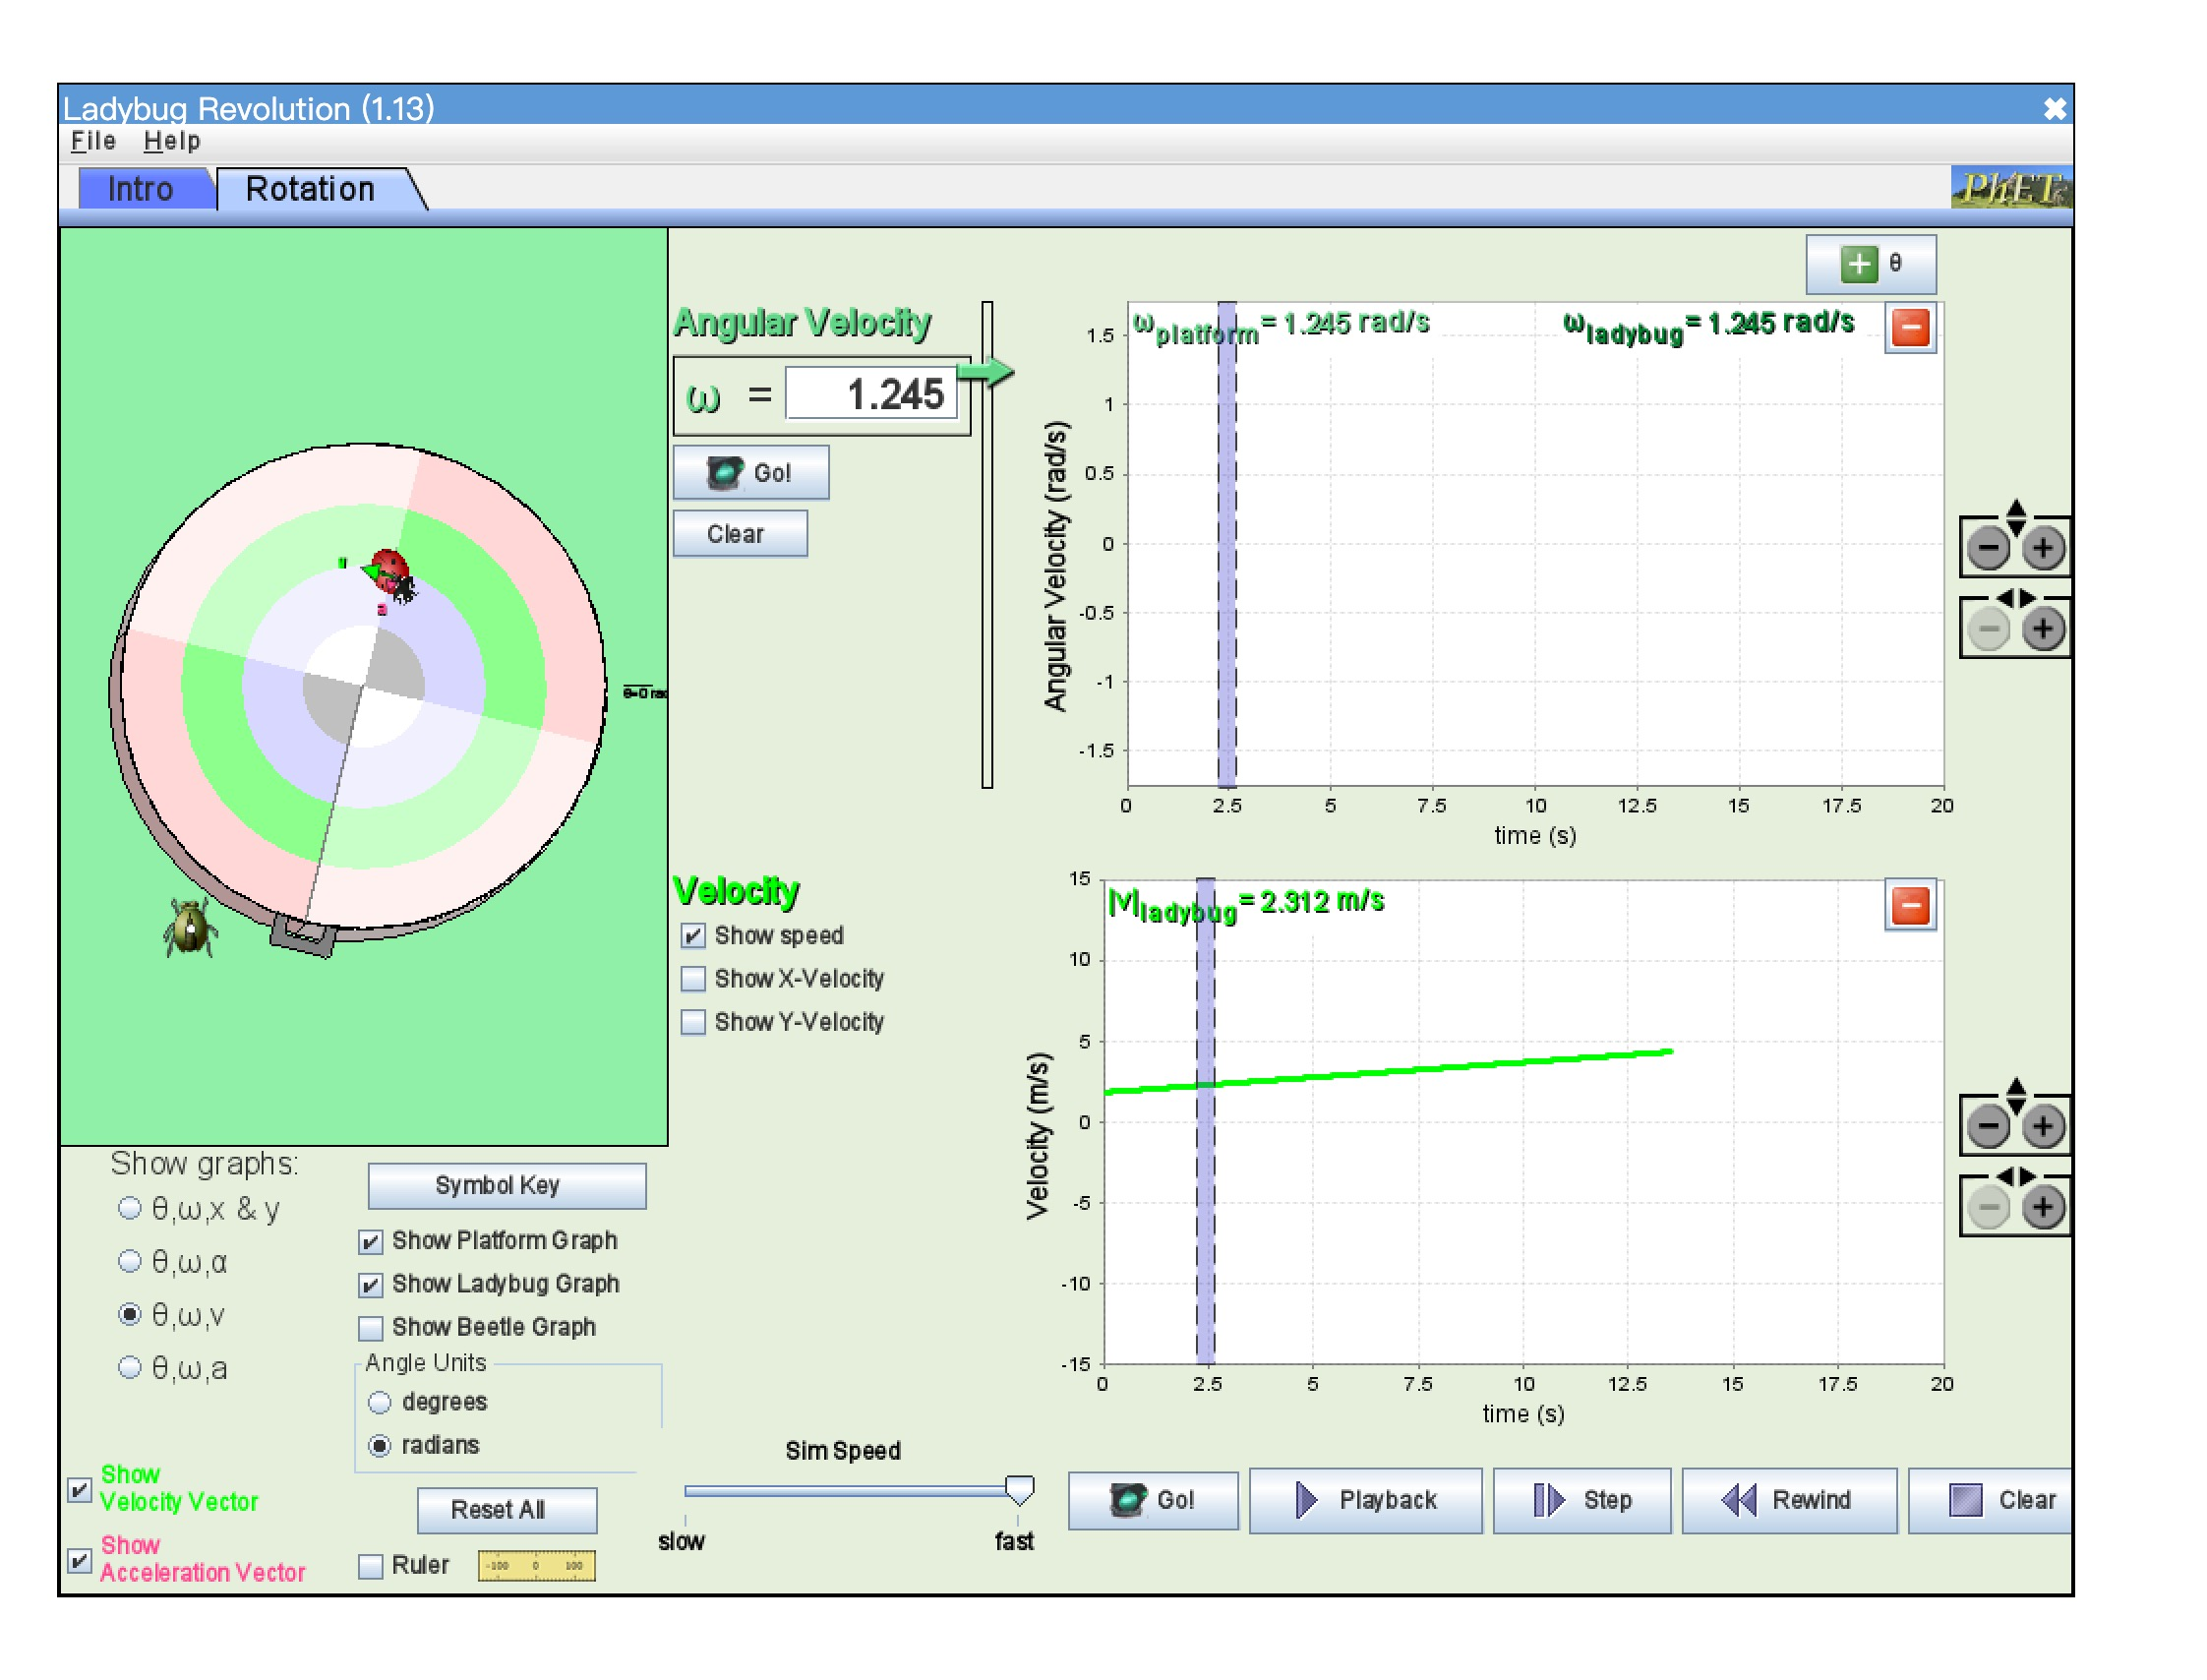
\includegraphics[width=0.3\textwidth]{2.jpeg}}
    \subfigure[$ 5.00s $]{
    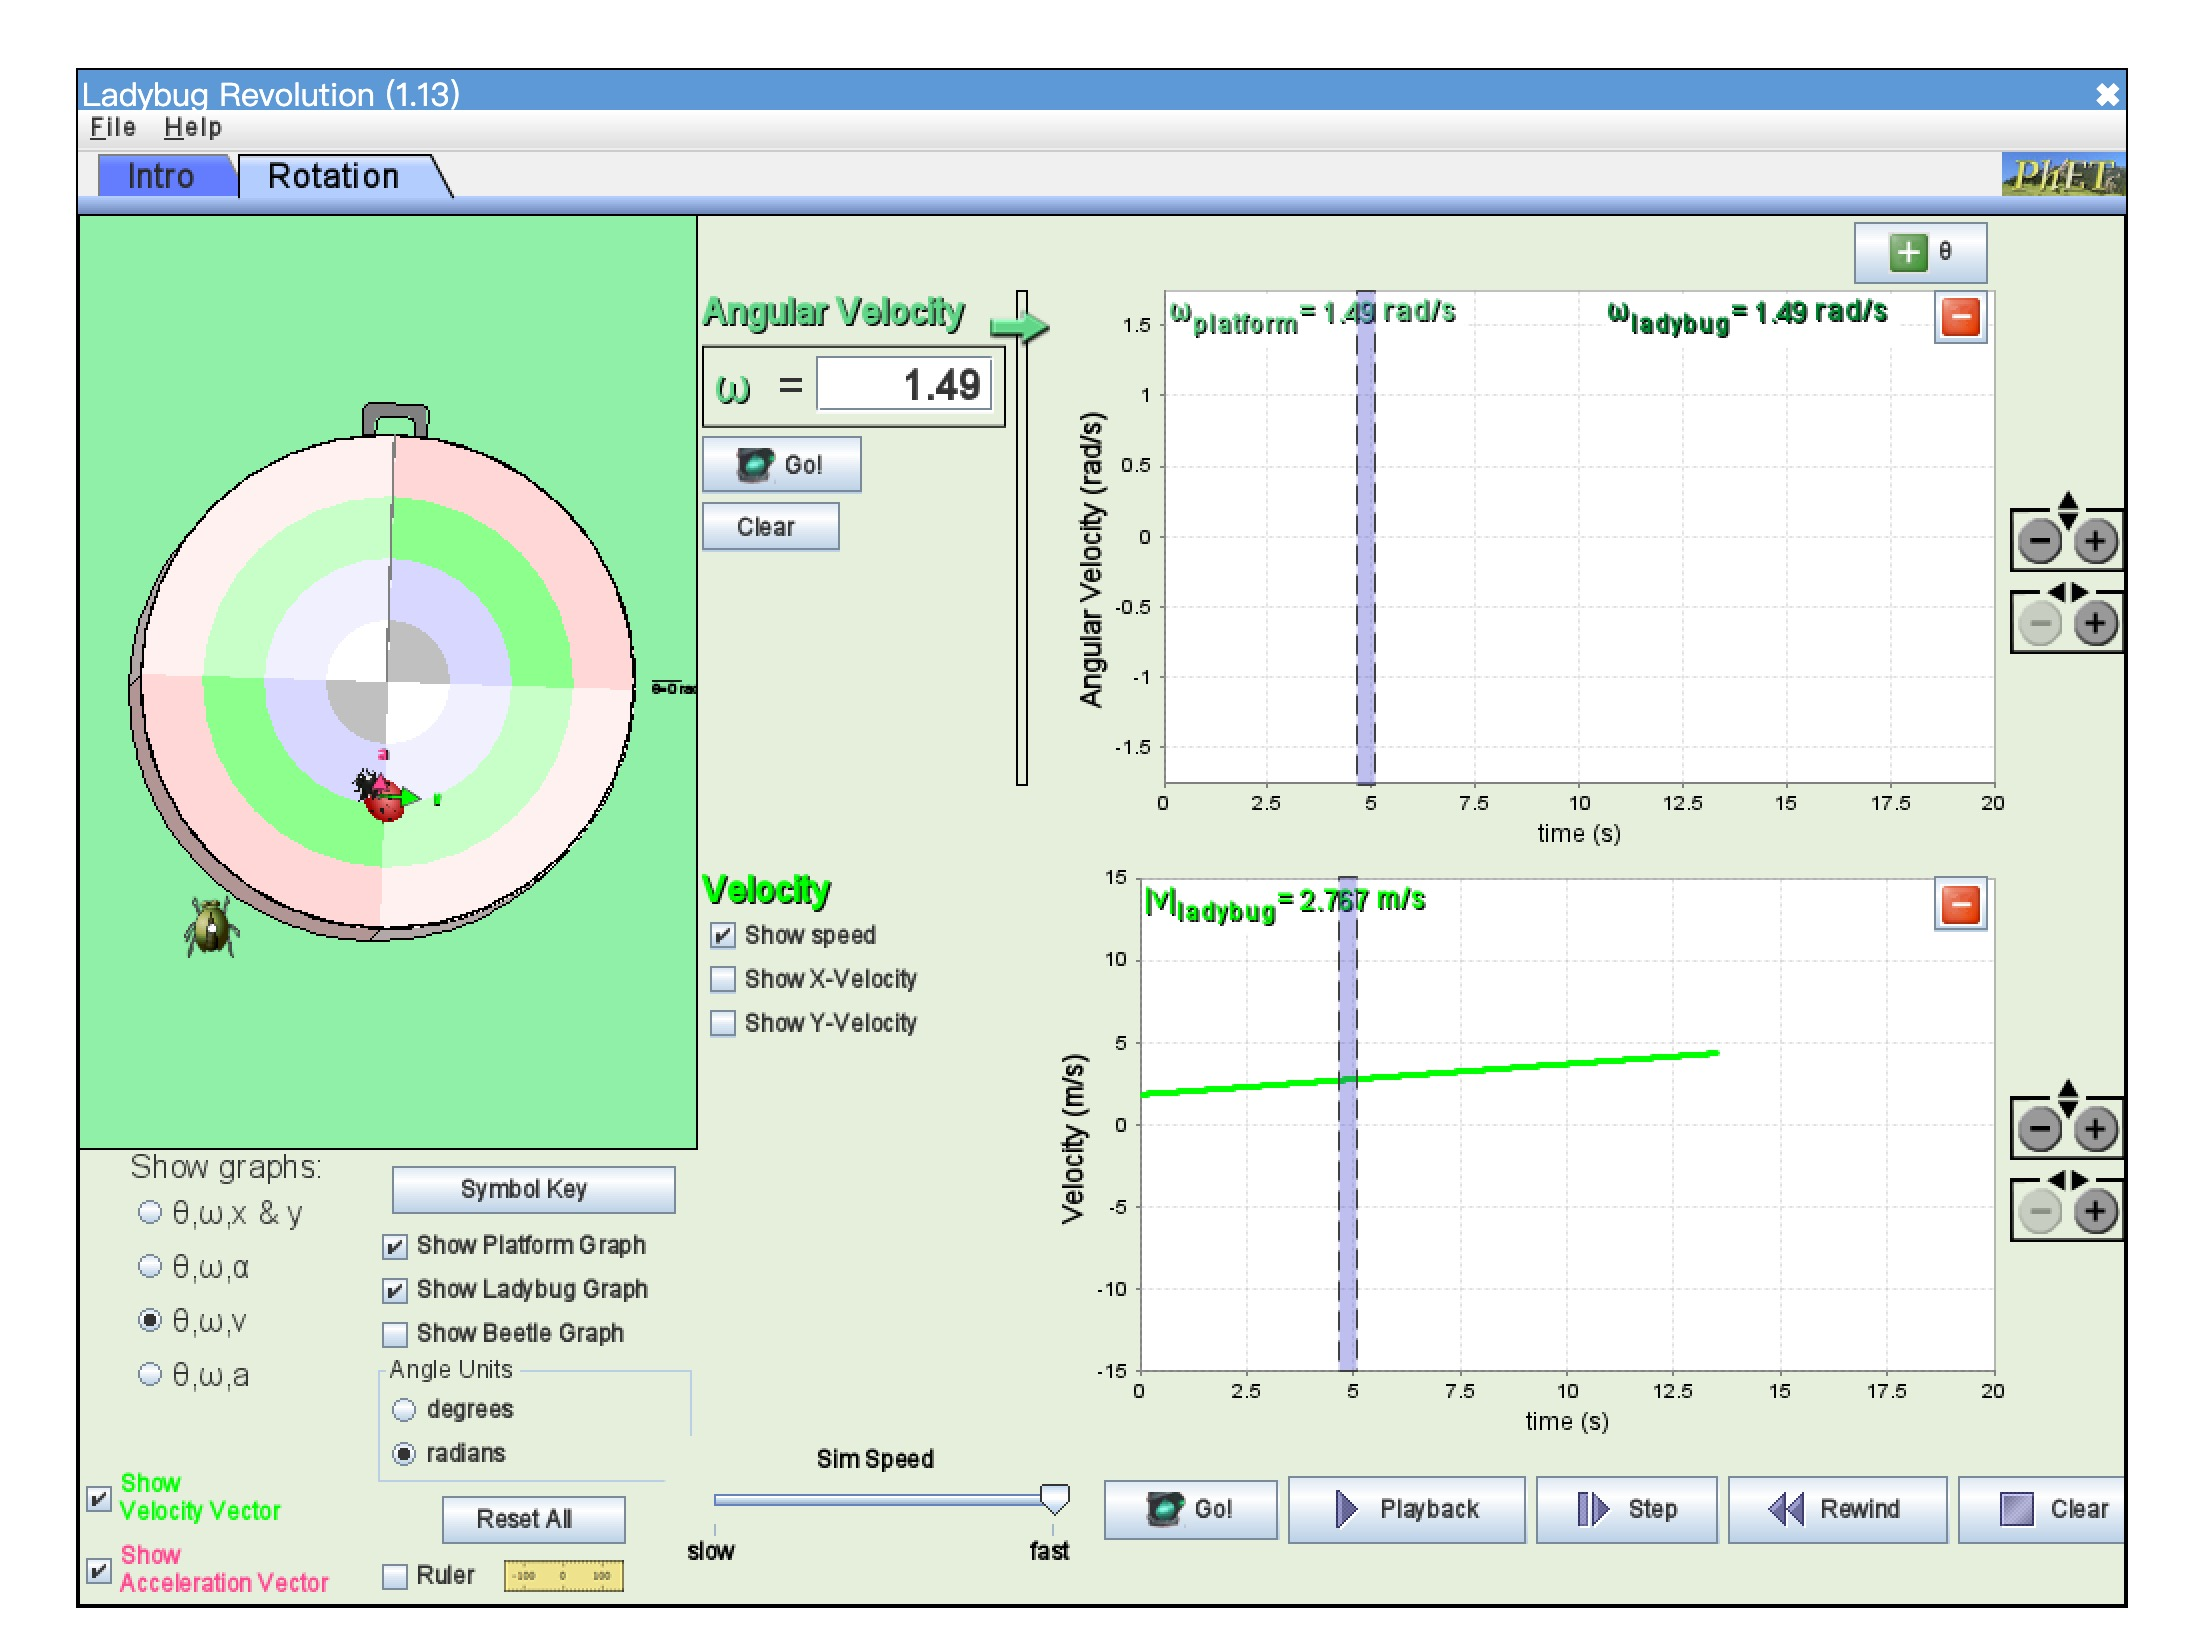
\includegraphics[width=0.3\textwidth]{3.jpeg}}
    \end{figure}
    \begin{figure}[H]
        \centering  %图片全局居中
        \subfigure[7.50$ s $]{
        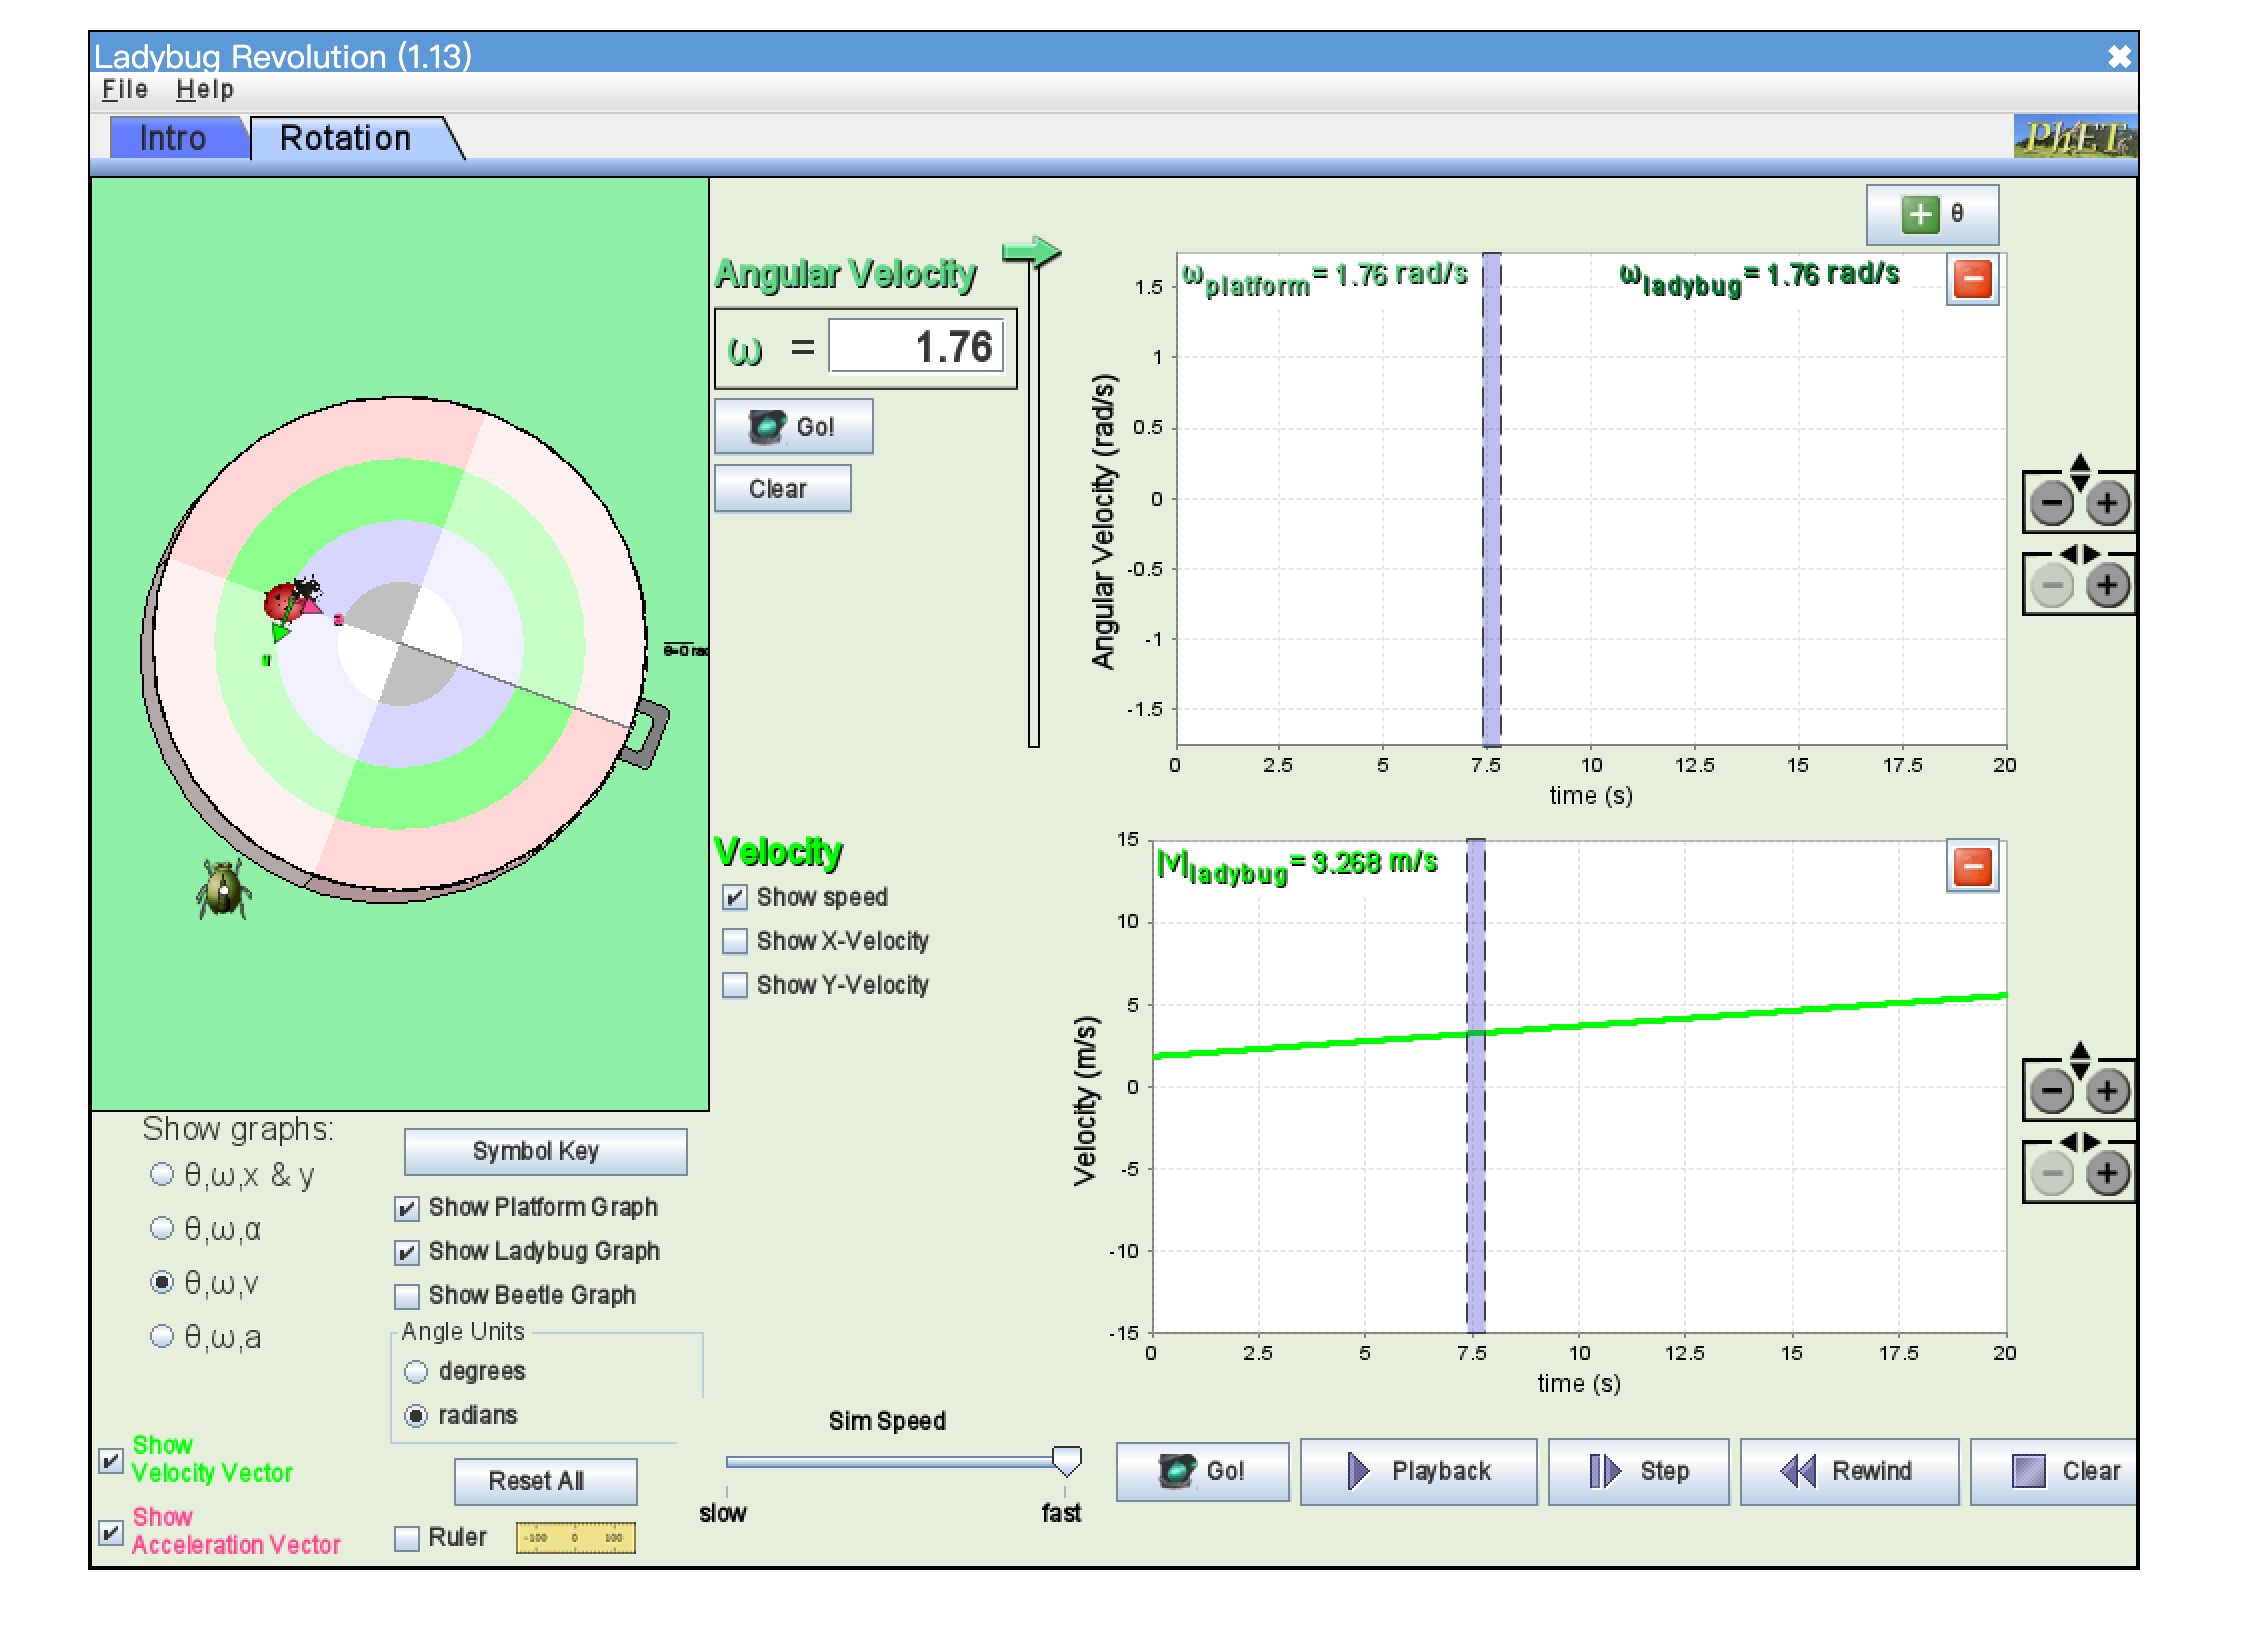
\includegraphics[width=0.3\textwidth]{4.jpeg}}
        \subfigure[$ 10.0s $]{
        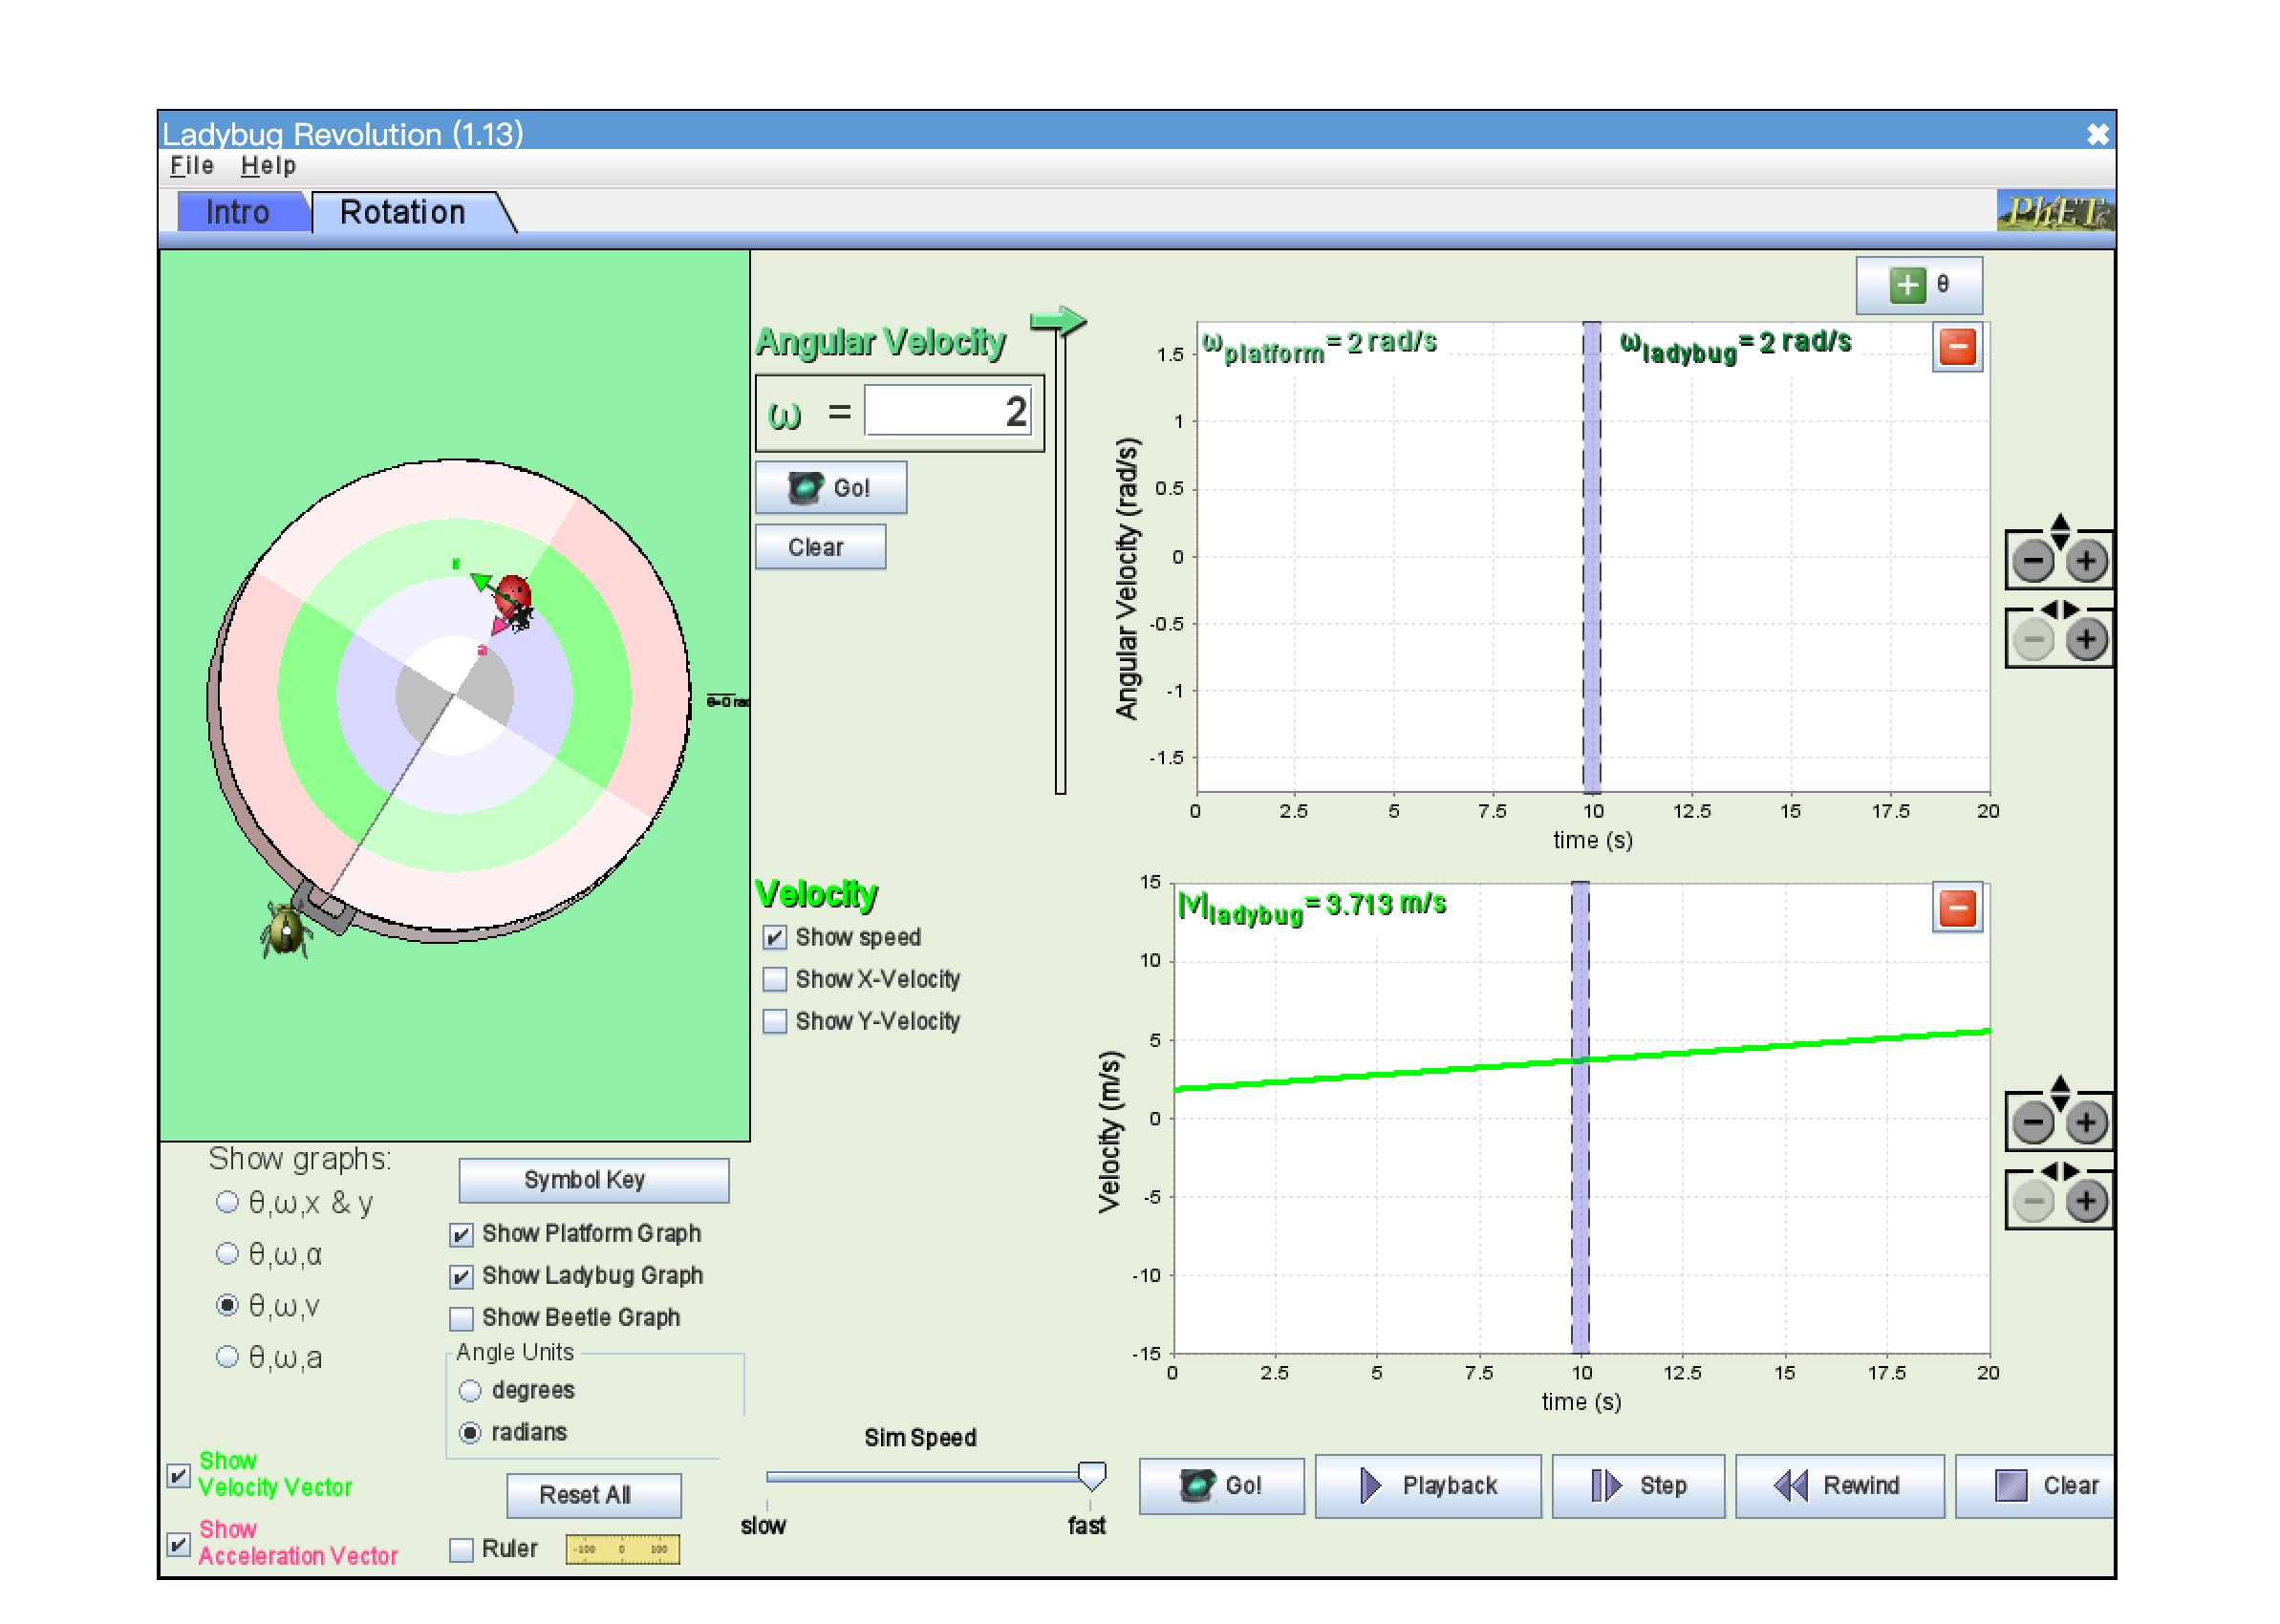
\includegraphics[width=0.3\textwidth]{5.jpeg}}
        \subfigure[$ 12.5s $]{
        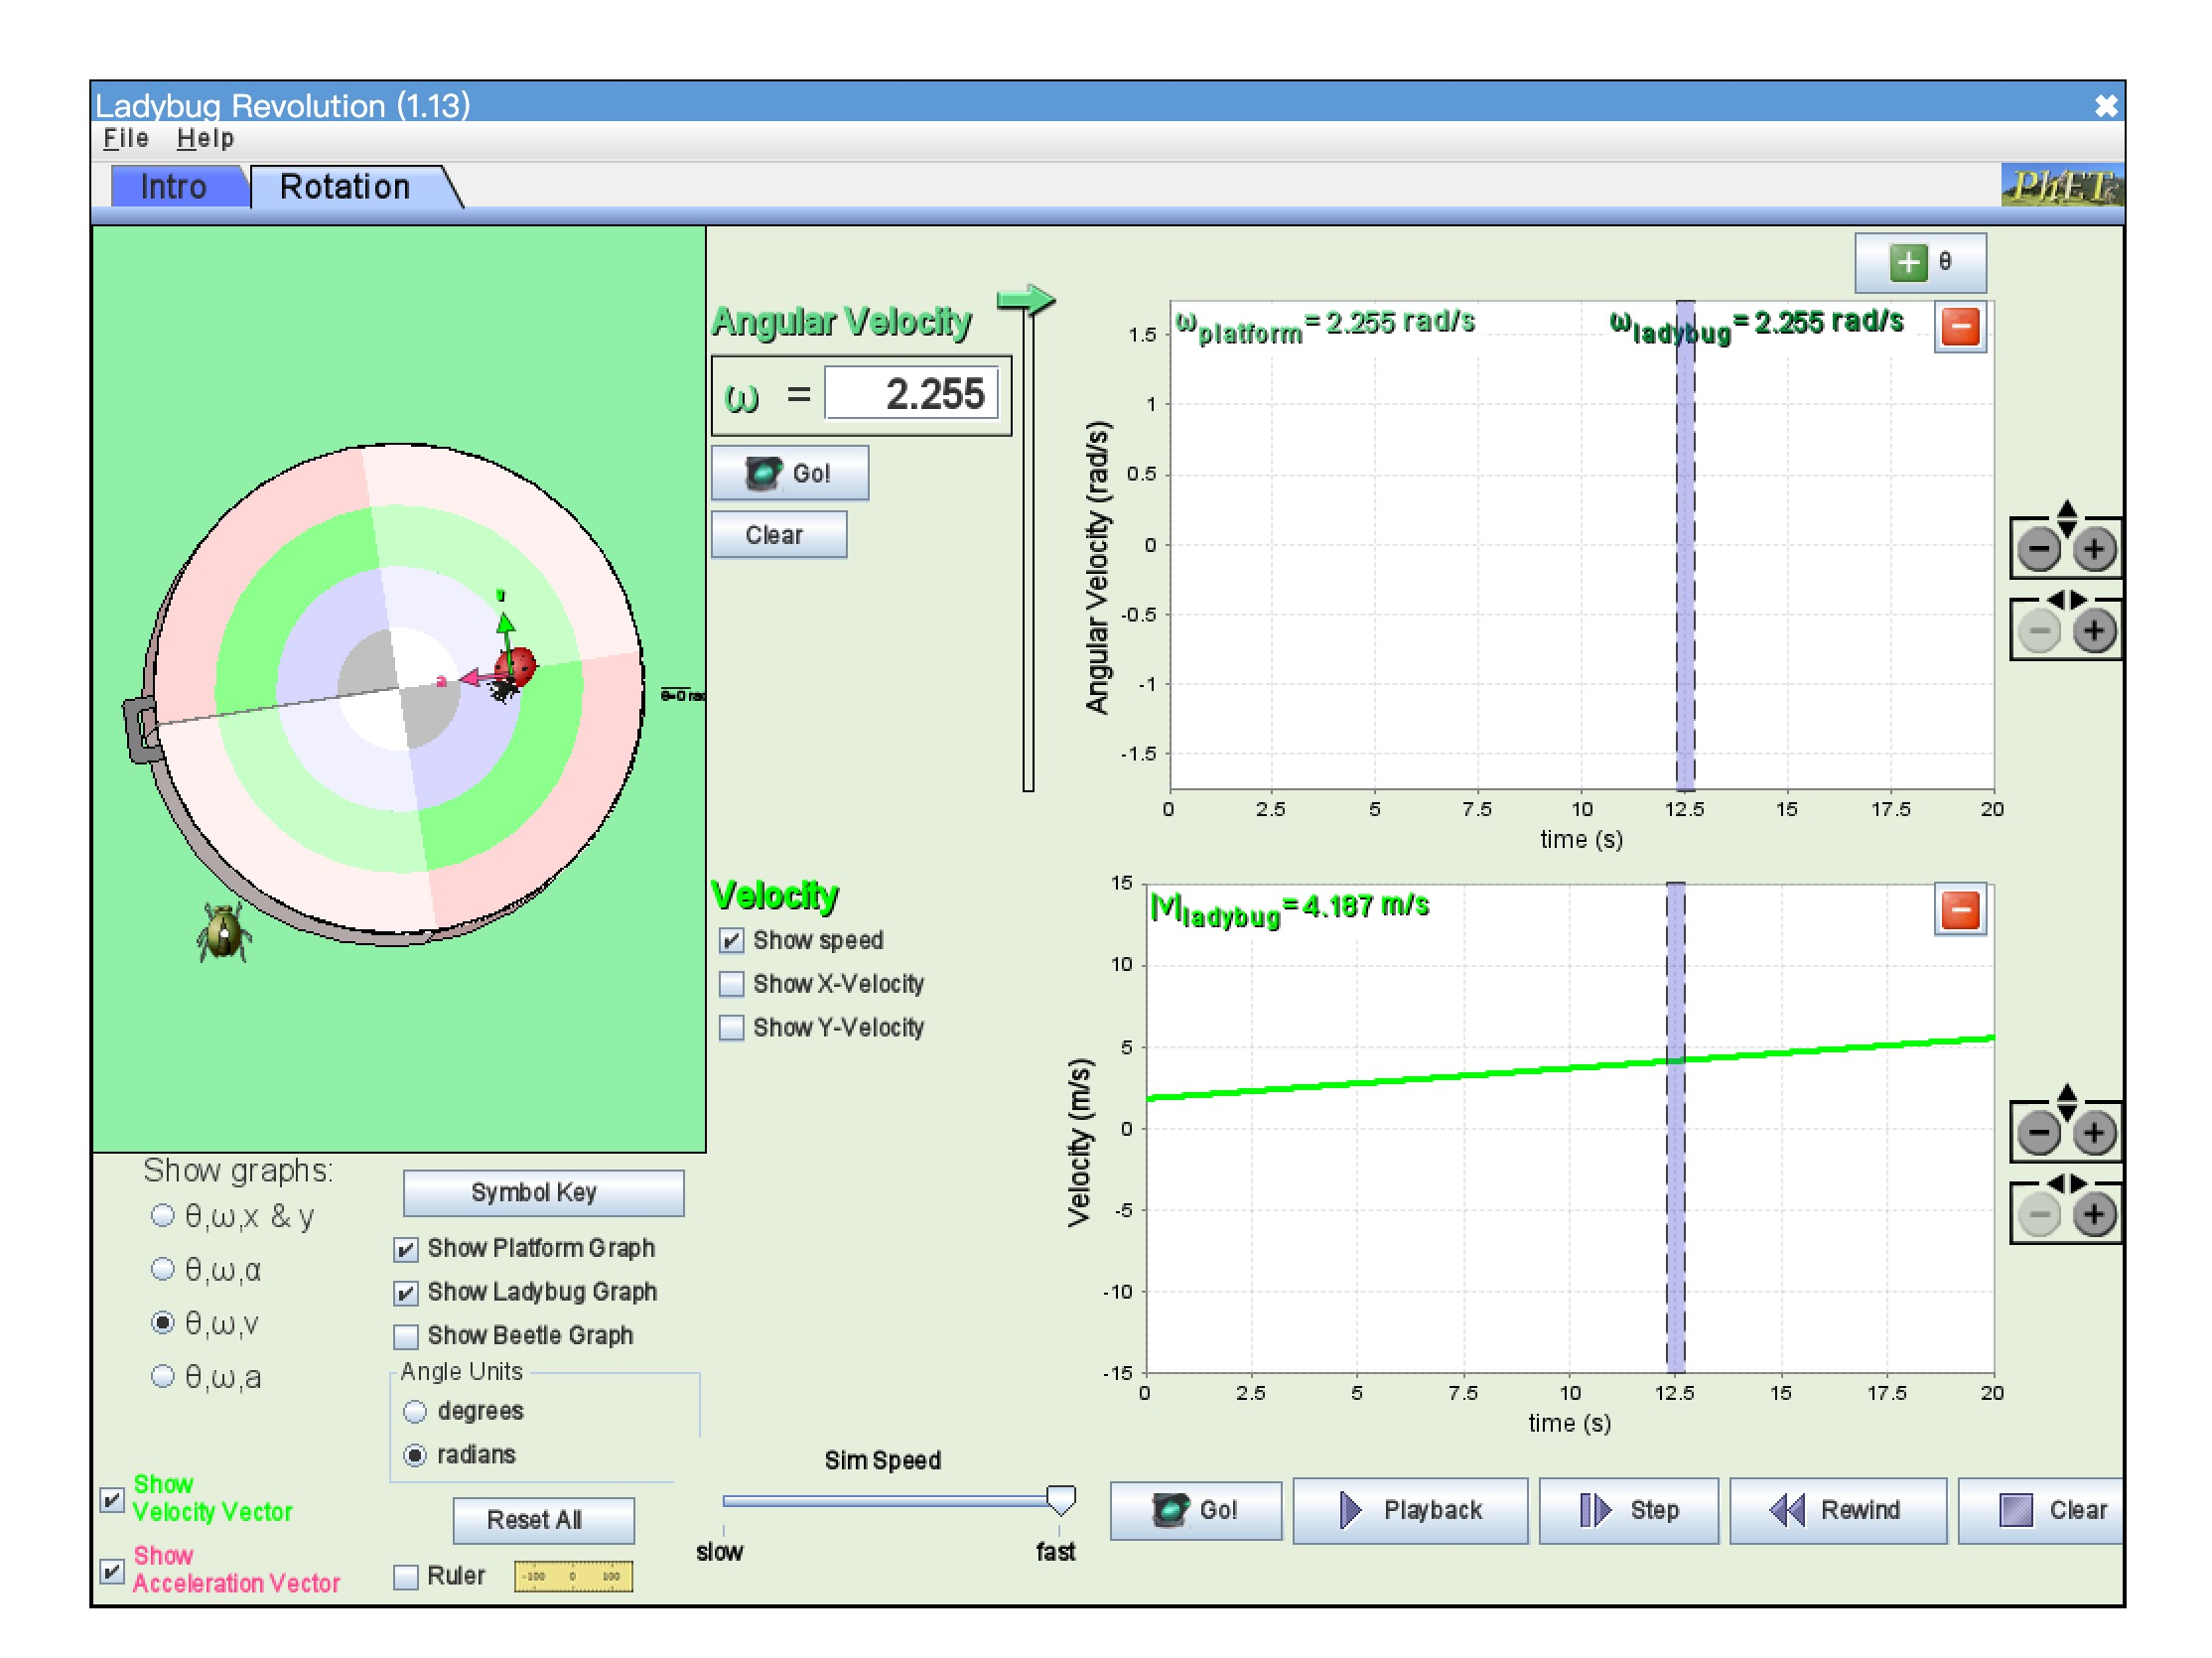
\includegraphics[width=0.3\textwidth]{6.jpeg}}
        \end{figure}
        \begin{figure}[H]
            \centering  %图片全局居中
            \subfigure[$ 15.0s $]{
            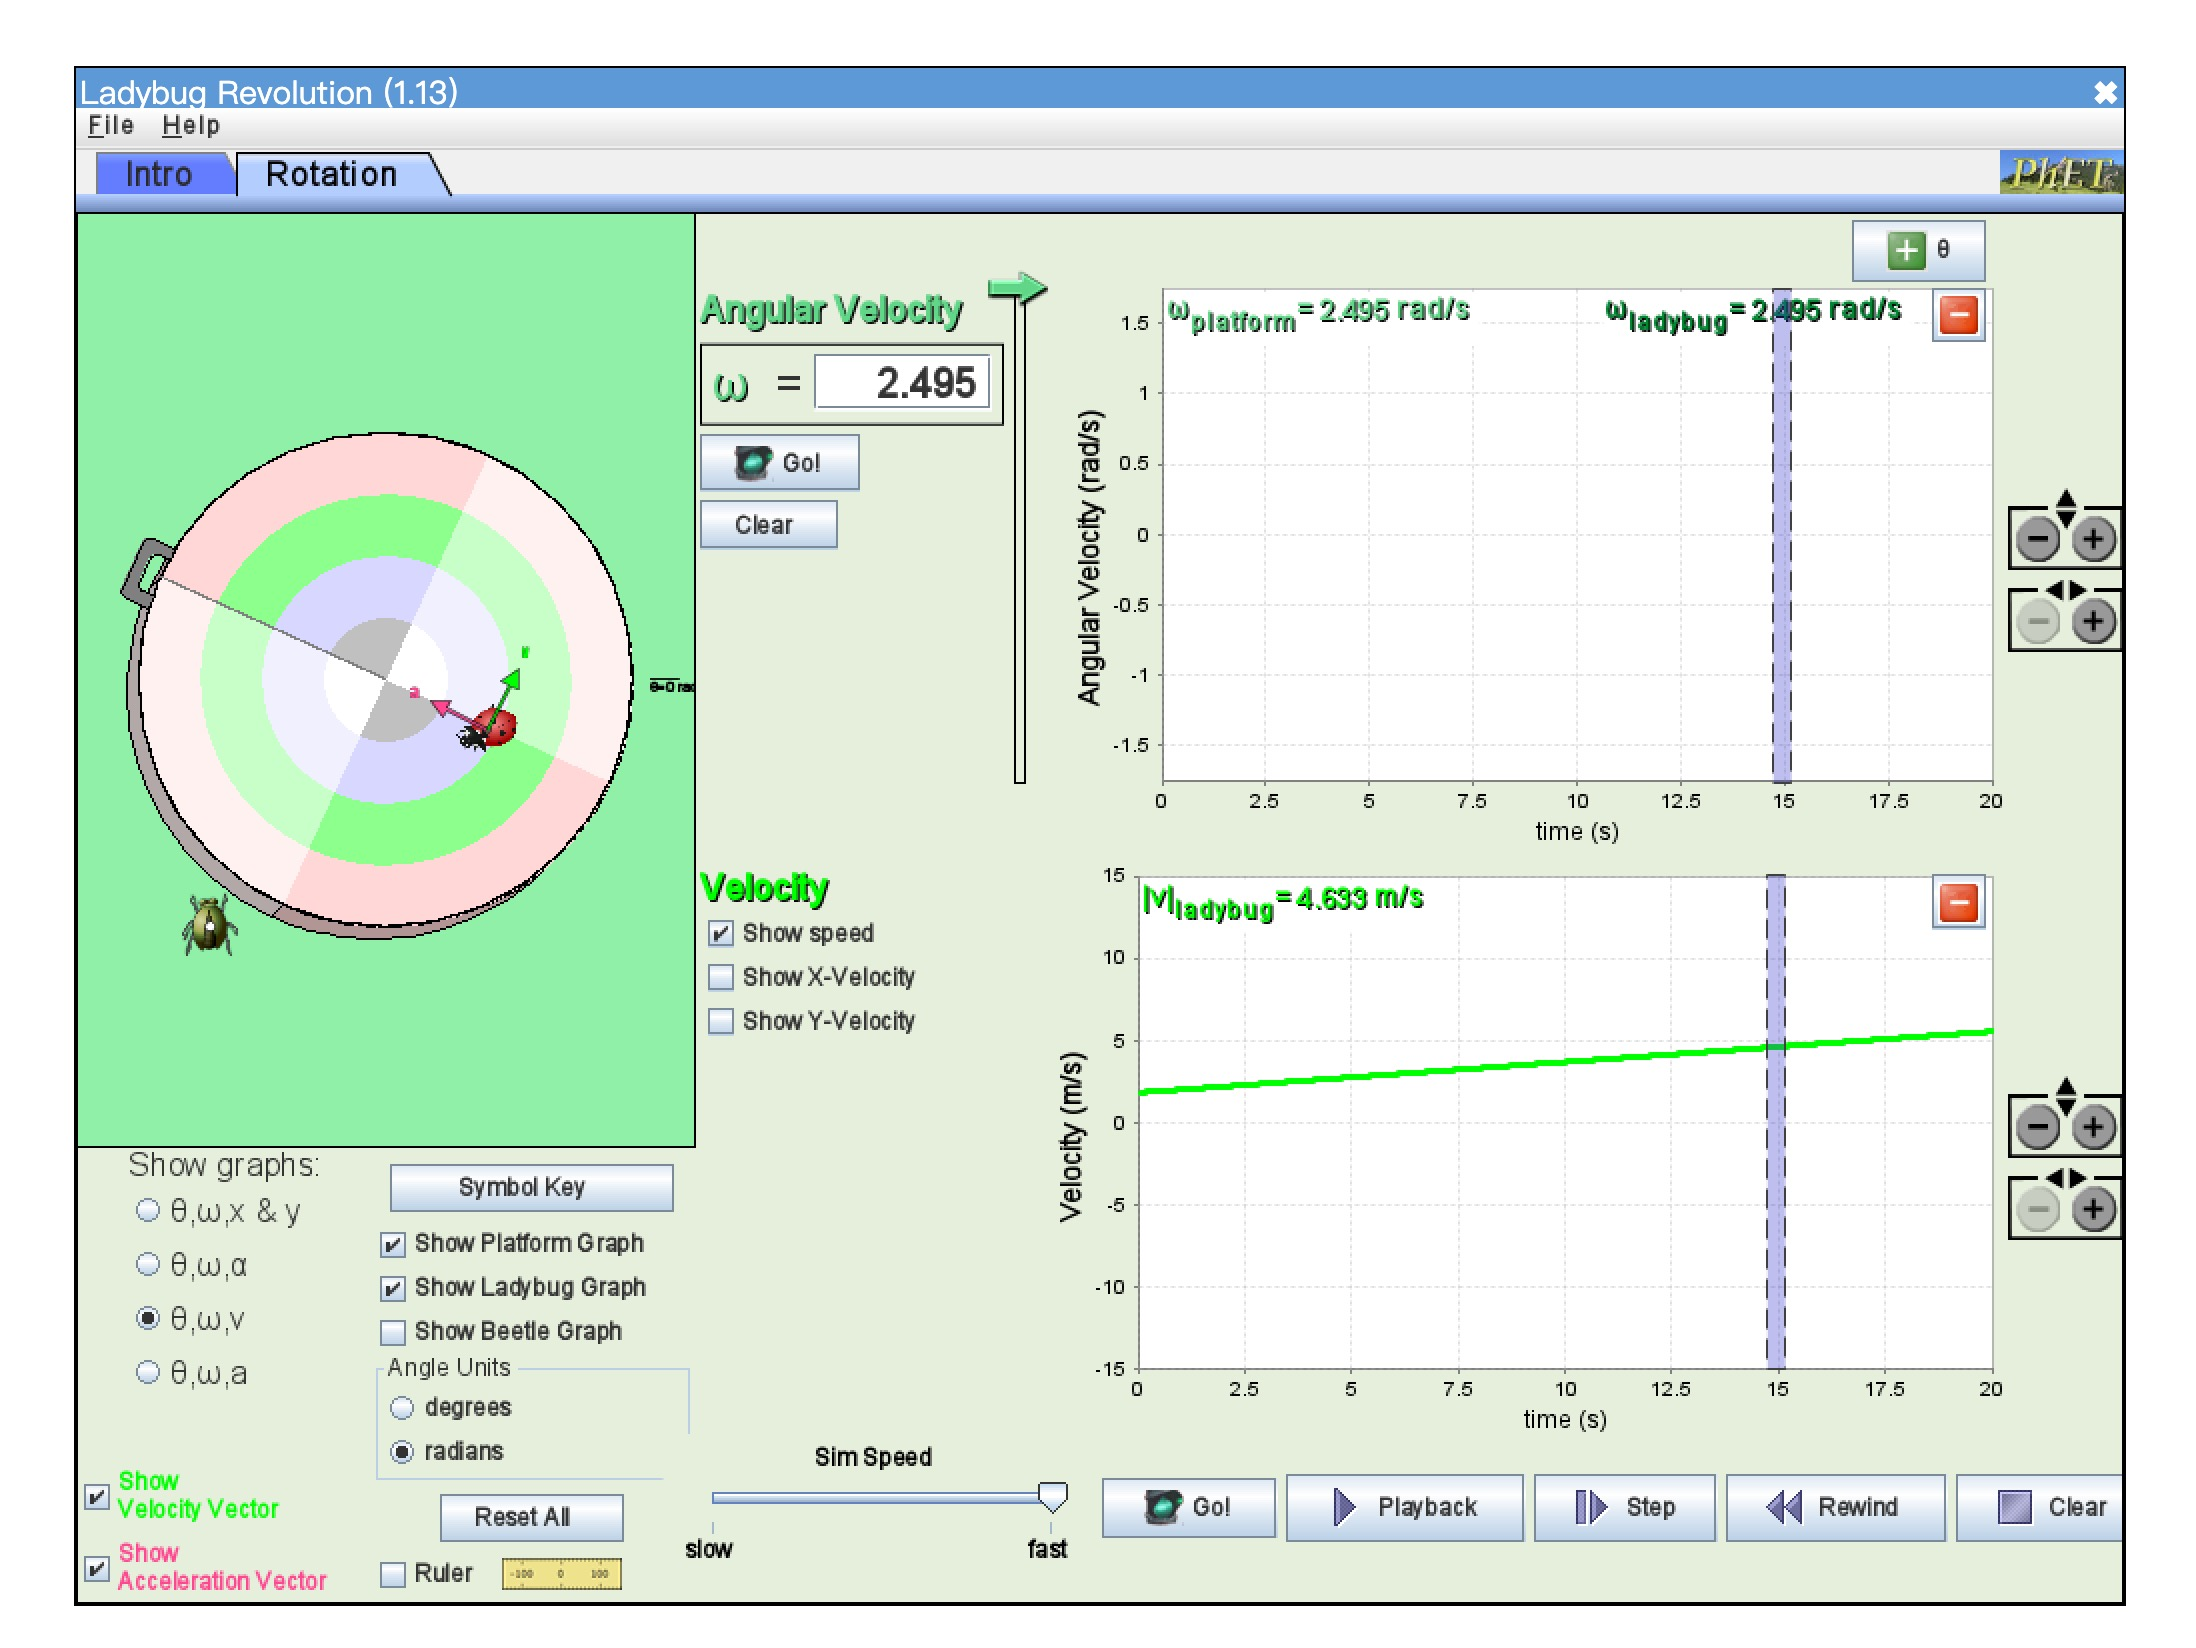
\includegraphics[width=0.3\textwidth]{7.jpeg}}
            \subfigure[$ 17.5s $]{
            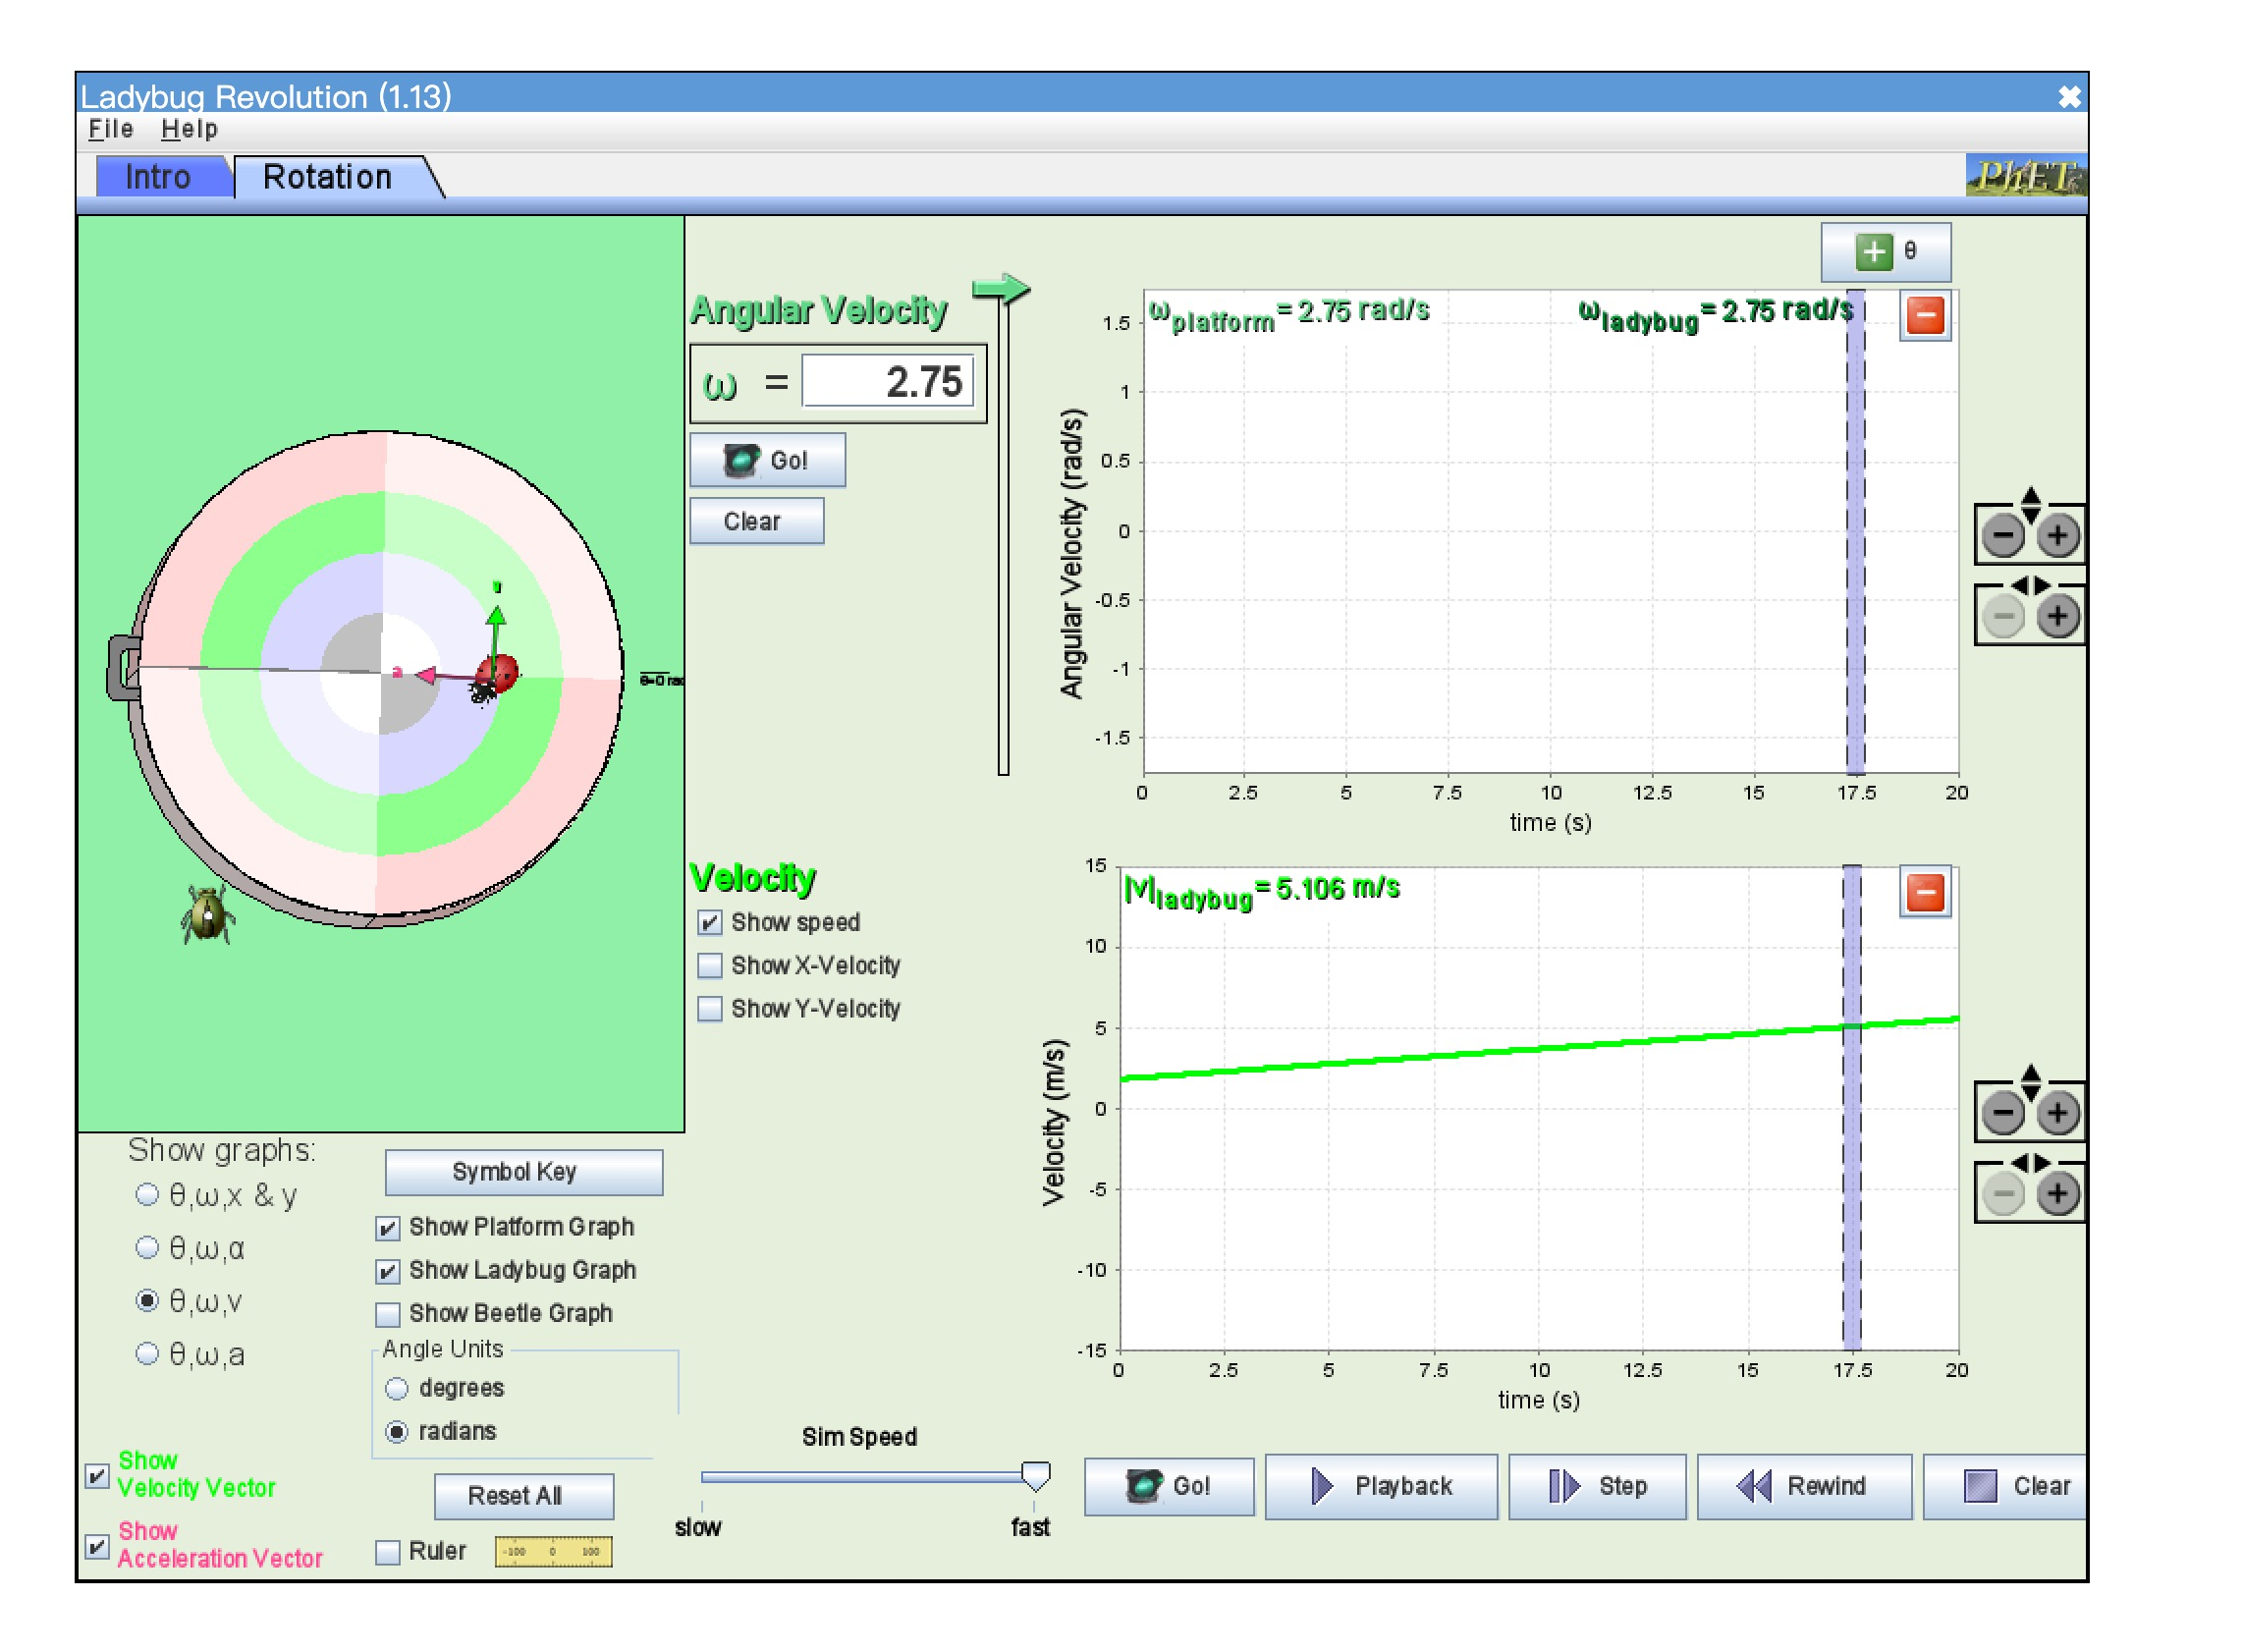
\includegraphics[width=0.3\textwidth]{8.jpeg}}
            \subfigure[$ 20.0s $]{
            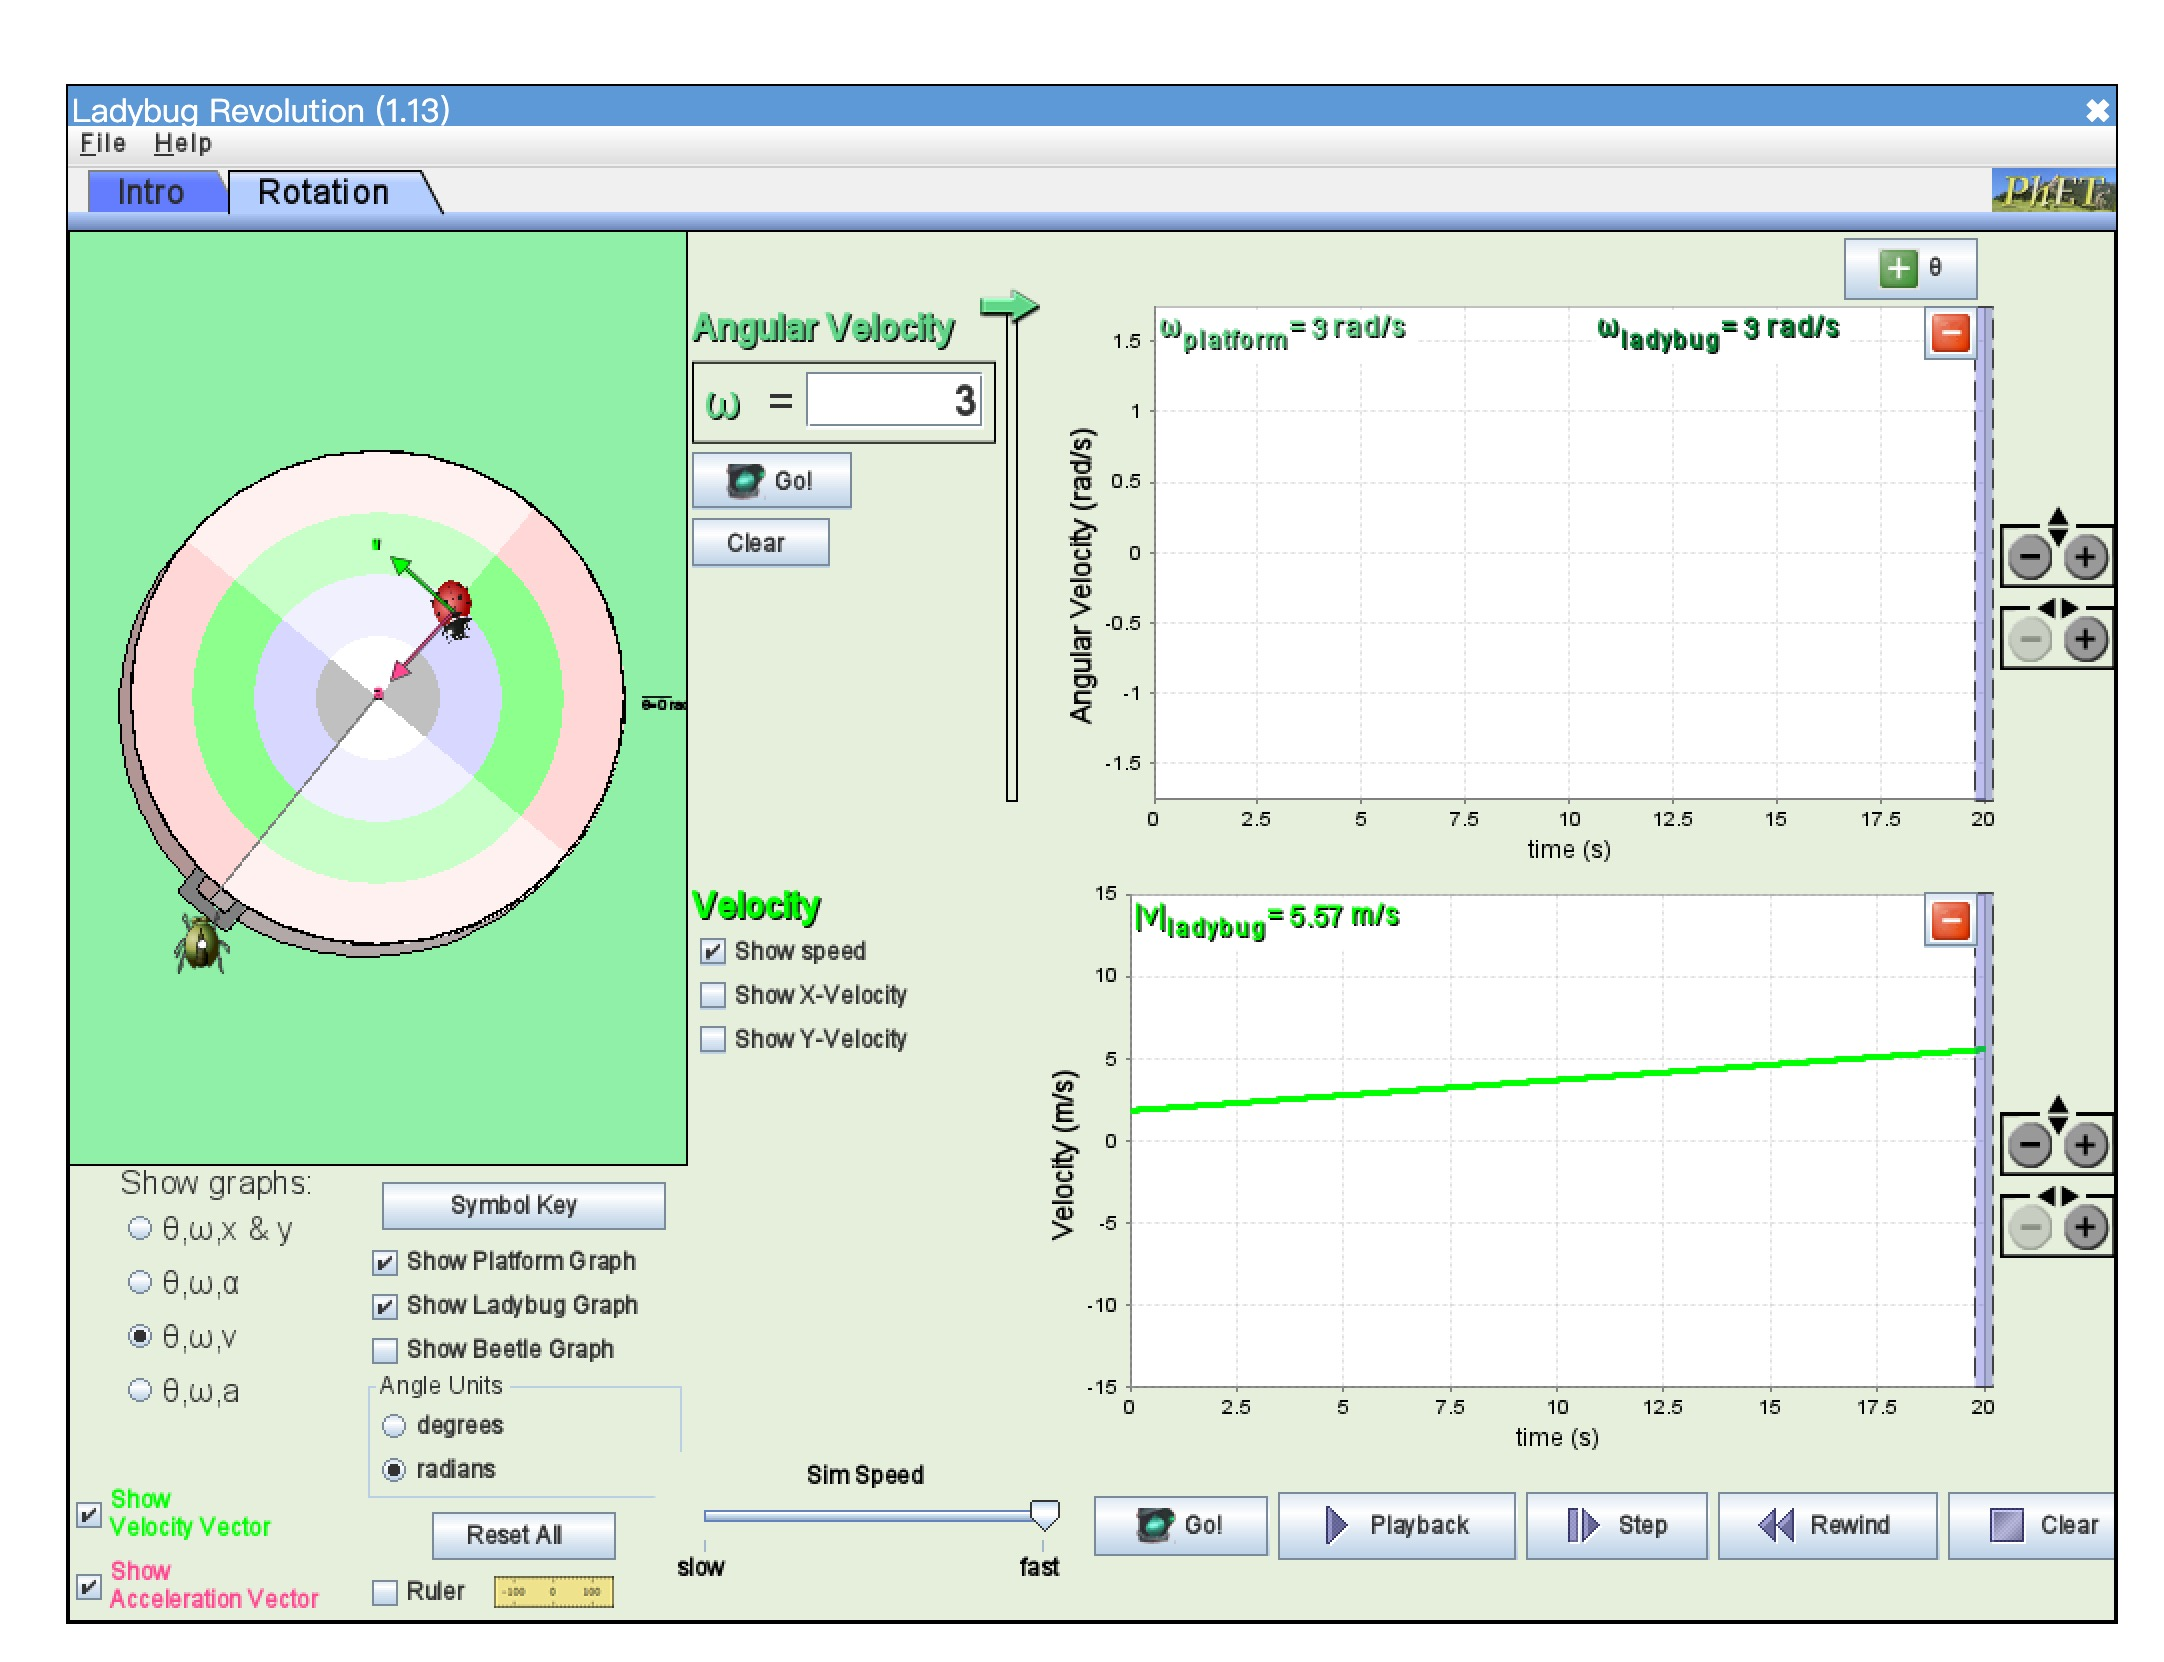
\includegraphics[width=0.3\textwidth]{9.jpeg}}
            \end{figure}
\subsection{Raw Data Table}
\begin{table}[!ht]
    \centering
    \begin{tabular}{|c|c|c|}
    \hline
        time($ s $) & $ \alpha $($ ms^{-2} $) & $ v $$(ms^{-1})$ \\ \hline
        0 & 0.1 & 1.866  \\ \hline
        2.50 & 0.1 & 2.312  \\ \hline
        5.00 & 0.1 & 2.767  \\ \hline
        7.50 & 0.1 & 3.268  \\ \hline
        10.0 & 0.1 & 3.713  \\ \hline
        12.5 & 0.1 & 4.187  \\ \hline
        15.0 & 0.1 & 4.633  \\ \hline
        17.5 & 0.1 & 5.106  \\ \hline
        20.0 & 0.1 & 5.57 \\ \hline
    \end{tabular}
    \caption{Raw Data Table}
\end{table}

\section{Data Processing}
Entering all the data into the data table, I drew a best-fit line with a slope of $ 0.1860 \pm 0.002 ms^{-2}$
\begin{figure}[H] %H为当前位置,!htb为忽略美学标准,htbp为浮动图形
    \centering %图片居中
    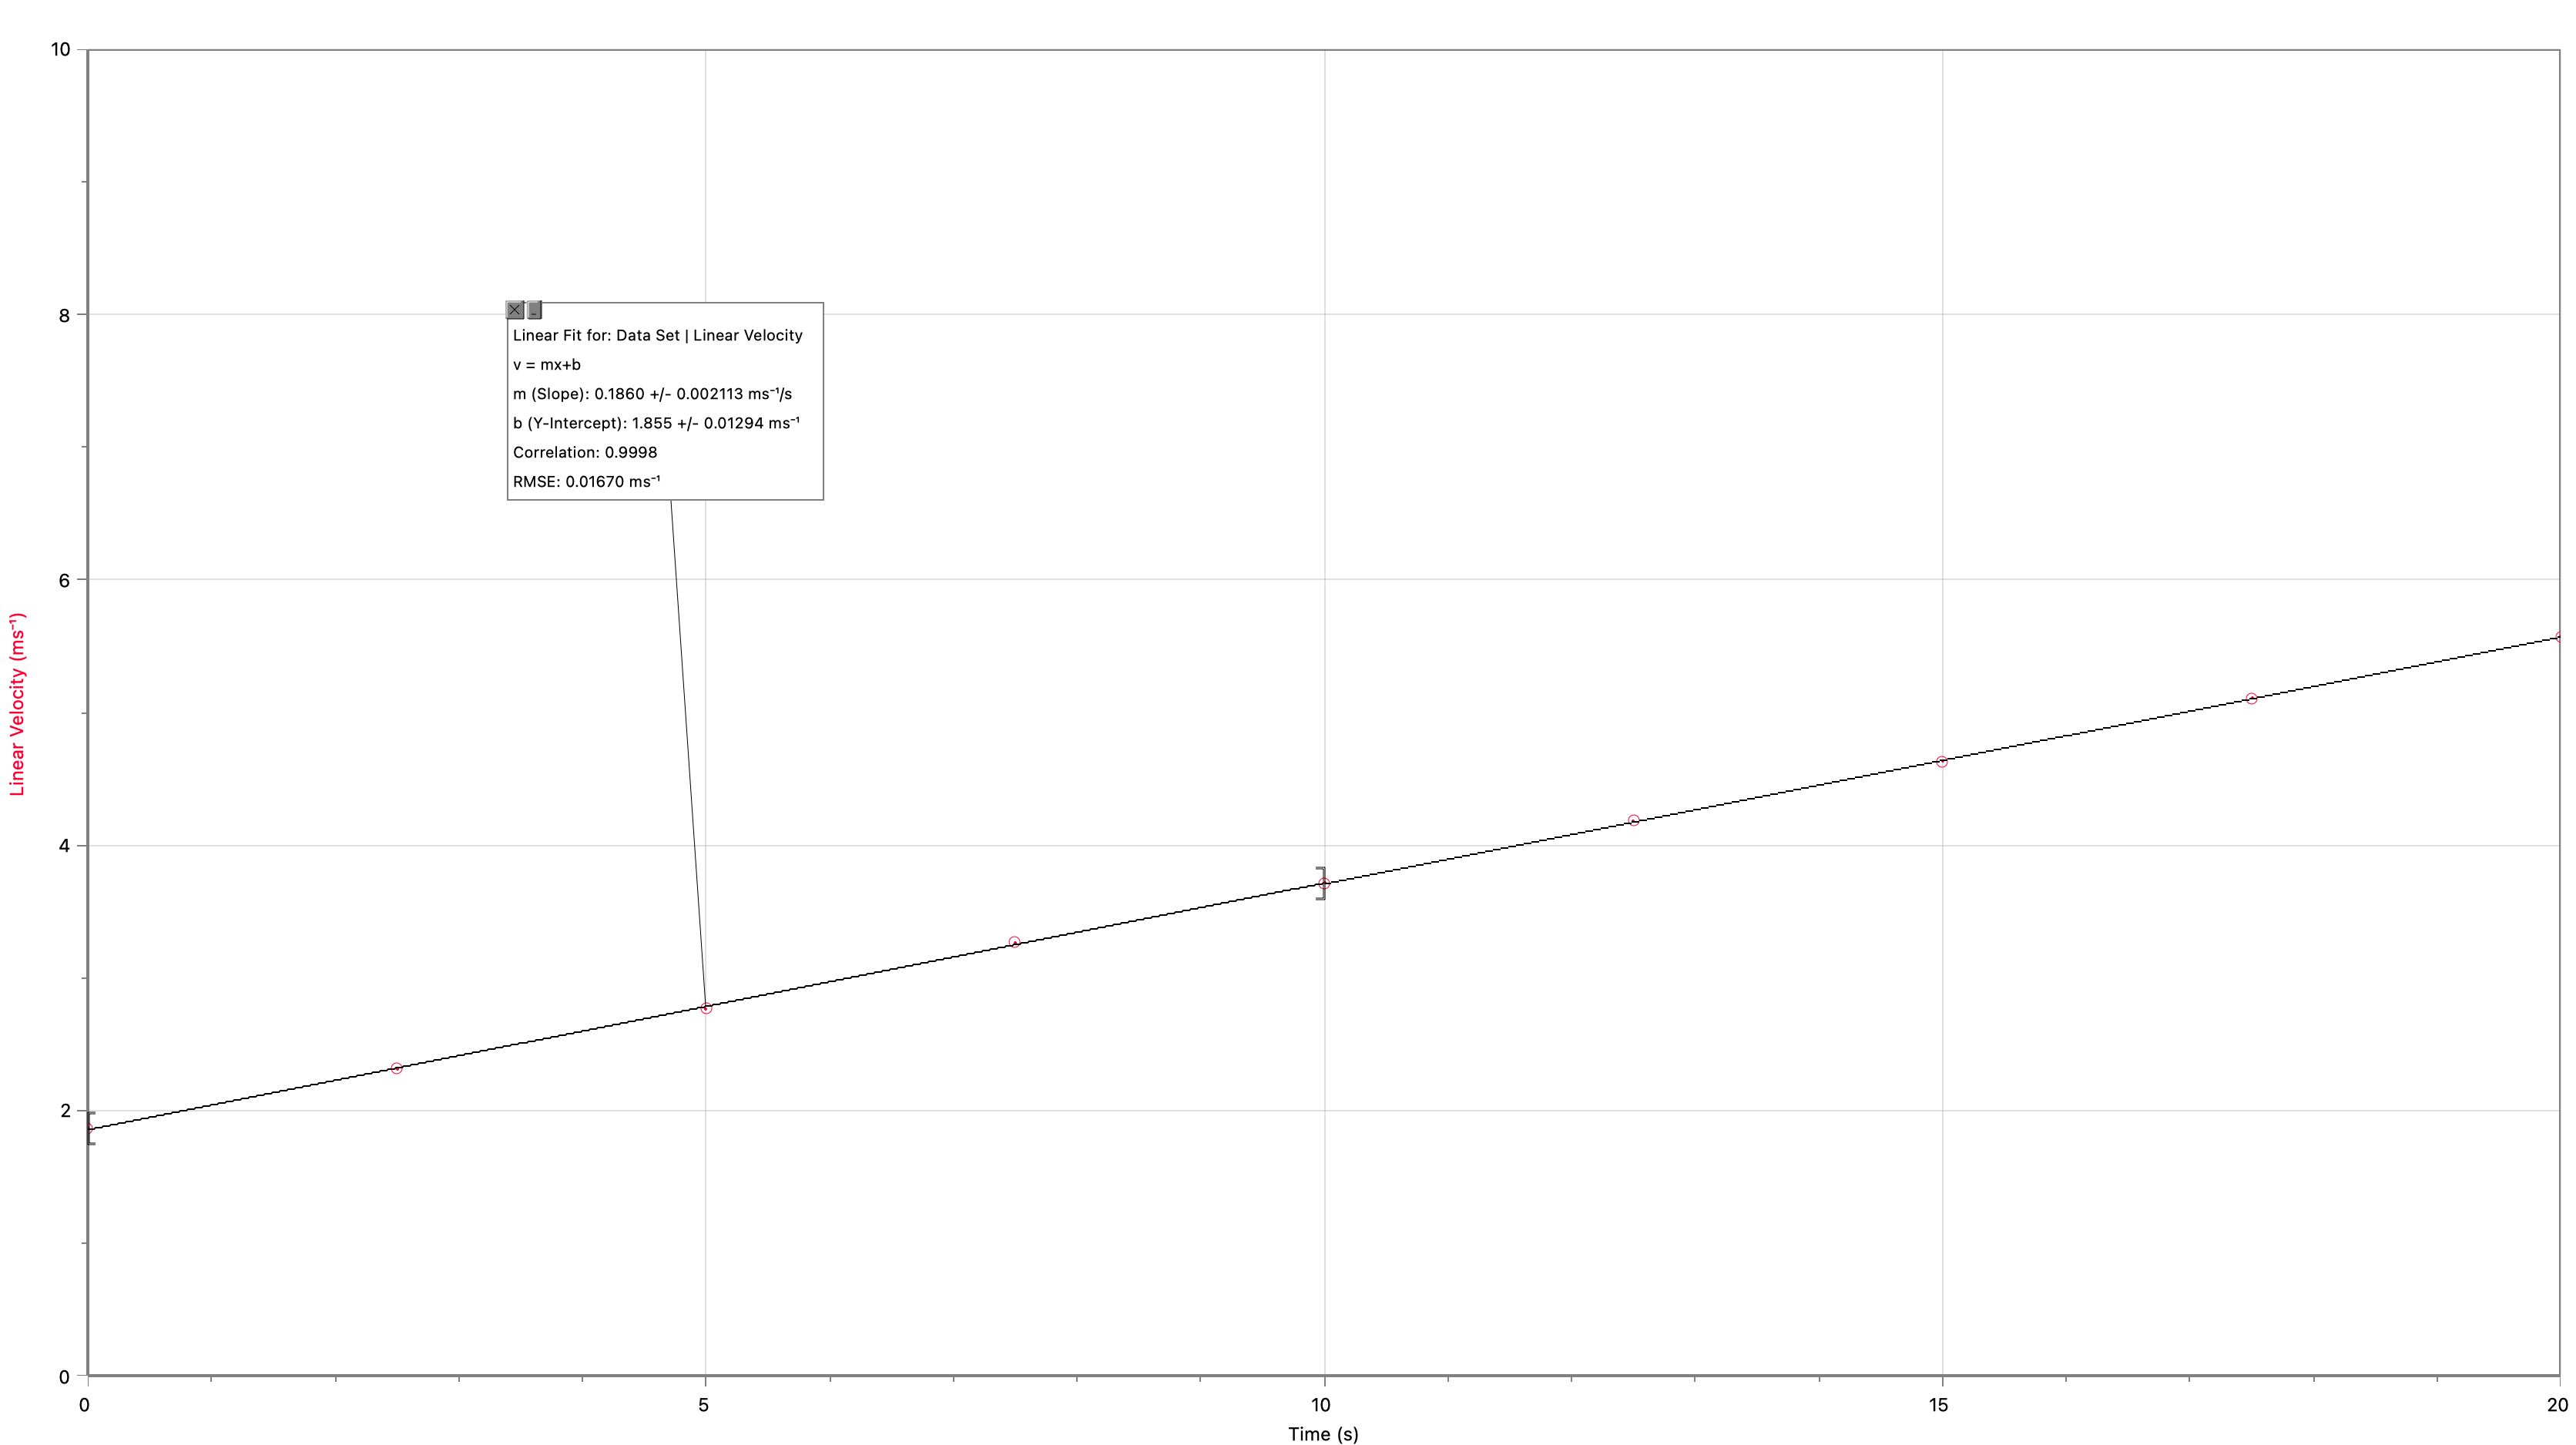
\includegraphics[width=\textwidth]{correlation.png}
    \caption{Relation Between $ t $ and $ v $} %最终文档中希望显示的图片标题
    \end{figure}
\section{Conclusion}
When an angular acceleration of 0.1 $ rads^{-2} $ is present, the correlation between linear velocity($ v $) and time($ t $) is \[
    v = 0.186t
\]\par
The Y-intercept of correlation is dismissed because the initial velocity for rotation was set to be $ 0.100 ms^{-2} $.\par
We can also deduce the numerical value through formulas.
Given that $ 
    v = r\omega
$ and $ \alpha = \frac{\Delta \omega}{\Delta t} $,
we can know that $ a = \frac{\Delta v}{\Delta t} = r\frac{\Delta \omega}{\Delta t} $. The radius of the rotation is about 1.86m, so the linear acceleration is supposed to be $ 0.186 ms^{-2}$.
\section{Evaluation}
This investigation is on simulation software, thus there's no uncertainty and very precise.
hi
\end{spacing}
\end{document}